\documentclass[a4paper,11pt,onecolumn,twoside]{article}
\usepackage{fancyhdr}
\usepackage{amsmath,amsfonts,amssymb}
\usepackage{graphicx}
\usepackage{fontspec}
\usepackage{booktabs}
\usepackage{indentfirst}
\usepackage{enumitem}
\usepackage{subfigure}
\usepackage{float}
\usepackage{caption}
\usepackage{graphicx}
% Please change the following fonts if they are not available.
\addtolength{\topmargin}{-54pt}
\setlength{\oddsidemargin}{-0.9cm}
\setlength{\evensidemargin}{\oddsidemargin}
\setlength{\textwidth}{17.00cm}
\setlength{\textheight}{24.50cm}
\usepackage{listings}
\usepackage{xcolor}
\usepackage[colorlinks,linkcolor=black,anchorcolor=black,citecolor=black]{hyperref}
\definecolor{dkgreen}{rgb}{0,0.6,0}
\definecolor{mauve}{rgb}{0.58,0,0.82}

\lstset{
	numbers=left,
	numberstyle=\tiny,
	stringstyle=\color{purple},
	basicstyle=\footnotesize\ttfamily, 
	keywordstyle=\color{blue}\bfseries,
	commentstyle=\color{olive},
	frame=shadowbox,
	%framerule=0pt,
	%backgroundcolor=\color{pink},
	rulesepcolor=\color{red!20!green!20!blue!20},
	%rulesepcolor=\color{brown}
	%xleftmargin=2em,xrightmargin=2em,aboveskip=1em
	escapeinside=``, 
	basicstyle=\tiny
}
\renewcommand{\baselinestretch}{1.1}
\parindent 22pt

\title{\Large \textbf{Data Analyzing with Logistic Regression and ANOVA}}
\author{
Mingyi Xue\footnote{Two authors are both exchange students from Nanjing University.}\\[2pt]
{\large \textit{School of Chemistry and Chemical Engineering, Nanjing University}}\\[6pt]
Wangqian Miao
\\[2pt]
{\large \textit{Kuang Yaming Hornors School, Biophysics, Nanjing University}}\\[6pt]
Instructor: Dr. Erin K. Melcon\\[2pt]
{\large \textit{Department of Statistics, University of California, Davis}}\\[2pt]
}
\date{}

\fancypagestyle{firststyle}
{
   \fancyhf{}
   \fancyhead[C]{STA101: Advanced Statistics For Biological Science, Course Project 1}
   \fancyhead[R]{\thepage}
}

\pagestyle{fancy}
\fancyhf{}
\fancyhead[LE,RO]{\thepage}
\fancyhead[CE]{STA101: Advanced Statistics For Biological Science}
\fancyhead[RE]{Project 2}
\fancyhead[CO]{M. Xue, W. Miao : Logistic Regression and ANOVA}
\fancyhead[LO]{}
\setlist{nolistsep}
\captionsetup{font=small}
\newcommand{\supercite}[1]{\textsuperscript{\cite{#1}}}
\begin{document}
\maketitle
\thispagestyle{firststyle}
\setlength{\oddsidemargin}{ 1cm}
\setlength{\evensidemargin}{\oddsidemargin}
\setlength{\textwidth}{15.50cm}
\vspace{-.8cm}
\setcounter{page}{1}
\setlength{\oddsidemargin}{-.5cm}  % 3.17cm - 1 inch
\setlength{\evensidemargin}{\oddsidemargin}
\setlength{\textwidth}{17.00cm}
\tableofcontents
\newpage
\section{Task 1: Logistic Regression}
\subsection{Introduction}
In this task, we applied the logistic regression model to analyze the dataset of ``prostate.csv" which contains the information from patients who are being assessed for prostate cancer.\par
Our goal is to build a binary-classification model to predict whether someone will be diagnosed with prostate cancer.
The full model is as follows and we did some improvement to make our model more efficient.
\begin{equation}
\ln\left(\frac{\hat{\pi}}{1-\hat{\pi}}\right)=\beta_0+\beta_1X_1+\beta_2X_2+\beta_3X_3+\beta_4X_4+\beta_5X_5+\beta_{6}X_6+\beta_{7}X_7+\varepsilon
\end{equation}
\par
A summary table is listed below to interpret these variables. 
\begin{table}[H]
	\centering
	\begin{tabular}{cccc}
		\midrule[1.5pt]
		Name& Variable &Variable Kind  & Units\\
		\hline
		\texttt{cancer}&$Y$ & Response  & 0/1\\
		\texttt{psa} &$X_1$& Numerical  & mg/ml  \\
		\texttt{c.vol}& $X_2$ &Numerical &cc  \\
		\texttt{weight}& $X_3$ & Numerical& gm \\
		\texttt{age}&$X_4$& Numerical  & years \\
		\texttt{benign}& $X_5$& Numerical  & cm$^{2}$ \\
		\texttt{inv}& $X_6$& Categorical  & invasion/no-invasion \\
		\texttt{cap}& $X_7$& Numerical  & cm \\
		\midrule[1.5pt]
	\end{tabular}
	\caption{A summary table for variables }
\end{table}
\begin{table}[H]
	\centering
	\begin{tabular}{ccccccc}
		\midrule[1.5pt]
		& $X_{1}$&$X_{2}$&$X_{3}$&$X_{4}$&$X_{5}$&$X_{7}$\\
		\hline
		Min &0.651   & 0.2592  & 10.70  &41.00  & 0.000 &0.0000\\
		Max &265.072  &45.6042 &450.34  &79.00  &10.278  &18.1741\\ 
		\midrule[1.5pt]
	\end{tabular}
	\caption{Reasonable range for numeric variables}
\end{table}
\subsection{Model Fitting}
Firstly, stepwise selection methods are employed to choose the best logistic regression model for the dataset, based on the criteria of AIC.\par
\begin{table}[H]
	\centering
	\begin{tabular}{cc}
		\midrule[1.5pt]
		Method&Selected Model\\
		\hline
		\texttt{Forward}&$logit(\hat{\pi}) \sim X_2 + X_1 + X_4$\\
		\texttt{Backward} &$logit(\hat{\pi}) \sim X_1 + X_2 + X_4$\\
		\texttt{Forward/Backward} &$logit(\hat{\pi}) \sim X_2 + X_1 + X_4$\\
		\texttt{Backward/Forward} &$logit(\hat{\pi}) \sim X_1 + X_2 + X_4$\\
		\midrule[1.5pt]
	\end{tabular}
	\caption{Stepwise selection results}
\end{table}
The best model selected by all stepwise methods correspond with each other. As a result, \texttt{psa}, \texttt{c.vol} and \texttt{age} will be included in the candidate model.\par
\begin{equation}
\ln\left(\frac{\hat{\pi}}{1-\hat{\pi}}\right)=-9.0529+0.04064X_{1}+0.11788X_{2}+0.08779X_{4}
\end{equation}
\begin{table}[H]
	\centering
	\begin{tabular}{cccc}
		\midrule[1.5pt]
		&$\hat{\beta}$&$\exp(\hat{\beta})$&Pr(>|z|)\\
		\hline 
		\texttt{Intercept} &-9.05285&0.00012&0.0145 \\ 
		\texttt{X1} &0.04064 & 1.04147&0.0596\\ 
		\texttt{X2} &0.11788 &1.12511&0.0244\\
		\texttt{X4} &0.08779 &1.09175&0.1073\\ 
		\midrule[1.5pt]
	\end{tabular}
	\caption{Coefficients of the candidate model}
\end{table}
\subsection{CI \& HT for $\beta_{i}$'s}
Then we applied t test for each $\beta_{i}$, where $i = 1, 2, 3$, to see whether $X_{i}$ can be dropped from the model or has a significant effect on $Y$.\par
\begin{itemize}
	\item $H_{0}$: $\beta{i} = 0$. 
	\item $H_{A}$: $\beta{i} \neq 0$.
\end{itemize}
\par
Test-statistic is $ts=(\hat{\beta_{i}}-0)/SE(\beta_{i})$, corresponding confidence intervals are listed as follows,\par
\begin{table}[H]
	\centering
	\begin{tabular}{ccc}
		\midrule[1.5pt]
		&$2.5\%$&$97.5\%$\\
		\hline 
		\texttt{X1} & 0.0069  &0.0878\\ 
		\texttt{X2} & 0.0169  &0.2260\\
		\texttt{X4} &-0.0128  &0.2022\\ 
		\midrule[1.5pt]
	\end{tabular}
	\caption{$95\%$ Confidence Intervals for $\hat{\beta}$'s}
\end{table}

\begin{table}[H]
	\centering
	\begin{tabular}{ccc}
		\midrule[1.5pt]
		&$2.5\%$&$97.5\%$\\
		\hline 
		\texttt{exp.X1}&1.0069 &1.0918\\
		\texttt{exp.X2}&1.0170 &1.2536\\
		\texttt{exp.X4}&0.9873 &1.2240\\
		\midrule[1.5pt]
	\end{tabular}
	\caption{$95\%$ Confidence Intervals for $\exp(\hat{\beta})$'s}
\end{table}

\subsection{Model Selection}
P-value for $\hat{\beta_{3}}$ equals $0.1073$, which is large enough for us to fail to reject $H_{0}$. Besides, CI for $\exp(\hat{\beta_{3}})$ contains 1, which suggests $X_{4}$ may not have a significant effect on $Y$. So we used Likelihood Ratio Test to decide whether $X_{4}$ should be dropped from the model.
\begin{itemize}
	\item $H_{0}$: $X_{4}$ can be dropped from the model. 
	\item $H_{A}$: $X_{4}$ cannot be dropped from the model.
\end{itemize}
\par
Test-statistic is $LR = -2(LL_{0}-LL_{A})\sim \chi^{2}(dof = 1)$. P-value equals $0.0896$ which is larger than 0.05 but less than $0.10$. It is not large enough for us to accept $H_{0}$. As a result, we decided not to drop $X_{4}$ from the final model.\par
Interpret of the p-value for Likelihood Ratio test above.
\begin{itemize}
	\item It means if we used the smaller model without infomation on age to predict the diagnosis of prostate cancer, we would observe our data or more extreme with the probability of 0.0896.
\end{itemize}
\par
In conclusion, the final model is $logit(\hat{\pi}) \sim X_{1}+X_{2}+X_{4}$.\par
\subsection{Model Diagnostics}
\subsubsection{Normality}
Because $Y$ is binomially distributed, standardized residuals should be approximately normally distributed.\par
\begin{equation}
r_{i} = \frac{y_{i}-\hat{\pi_{i}}}{\sqrt{\hat\pi_{i}(1-\hat{\pi_{i}})(1-h_{ii})n_{1}}}\sim N(0,1)
\end{equation}
\begin{figure}[H]
	\centering
	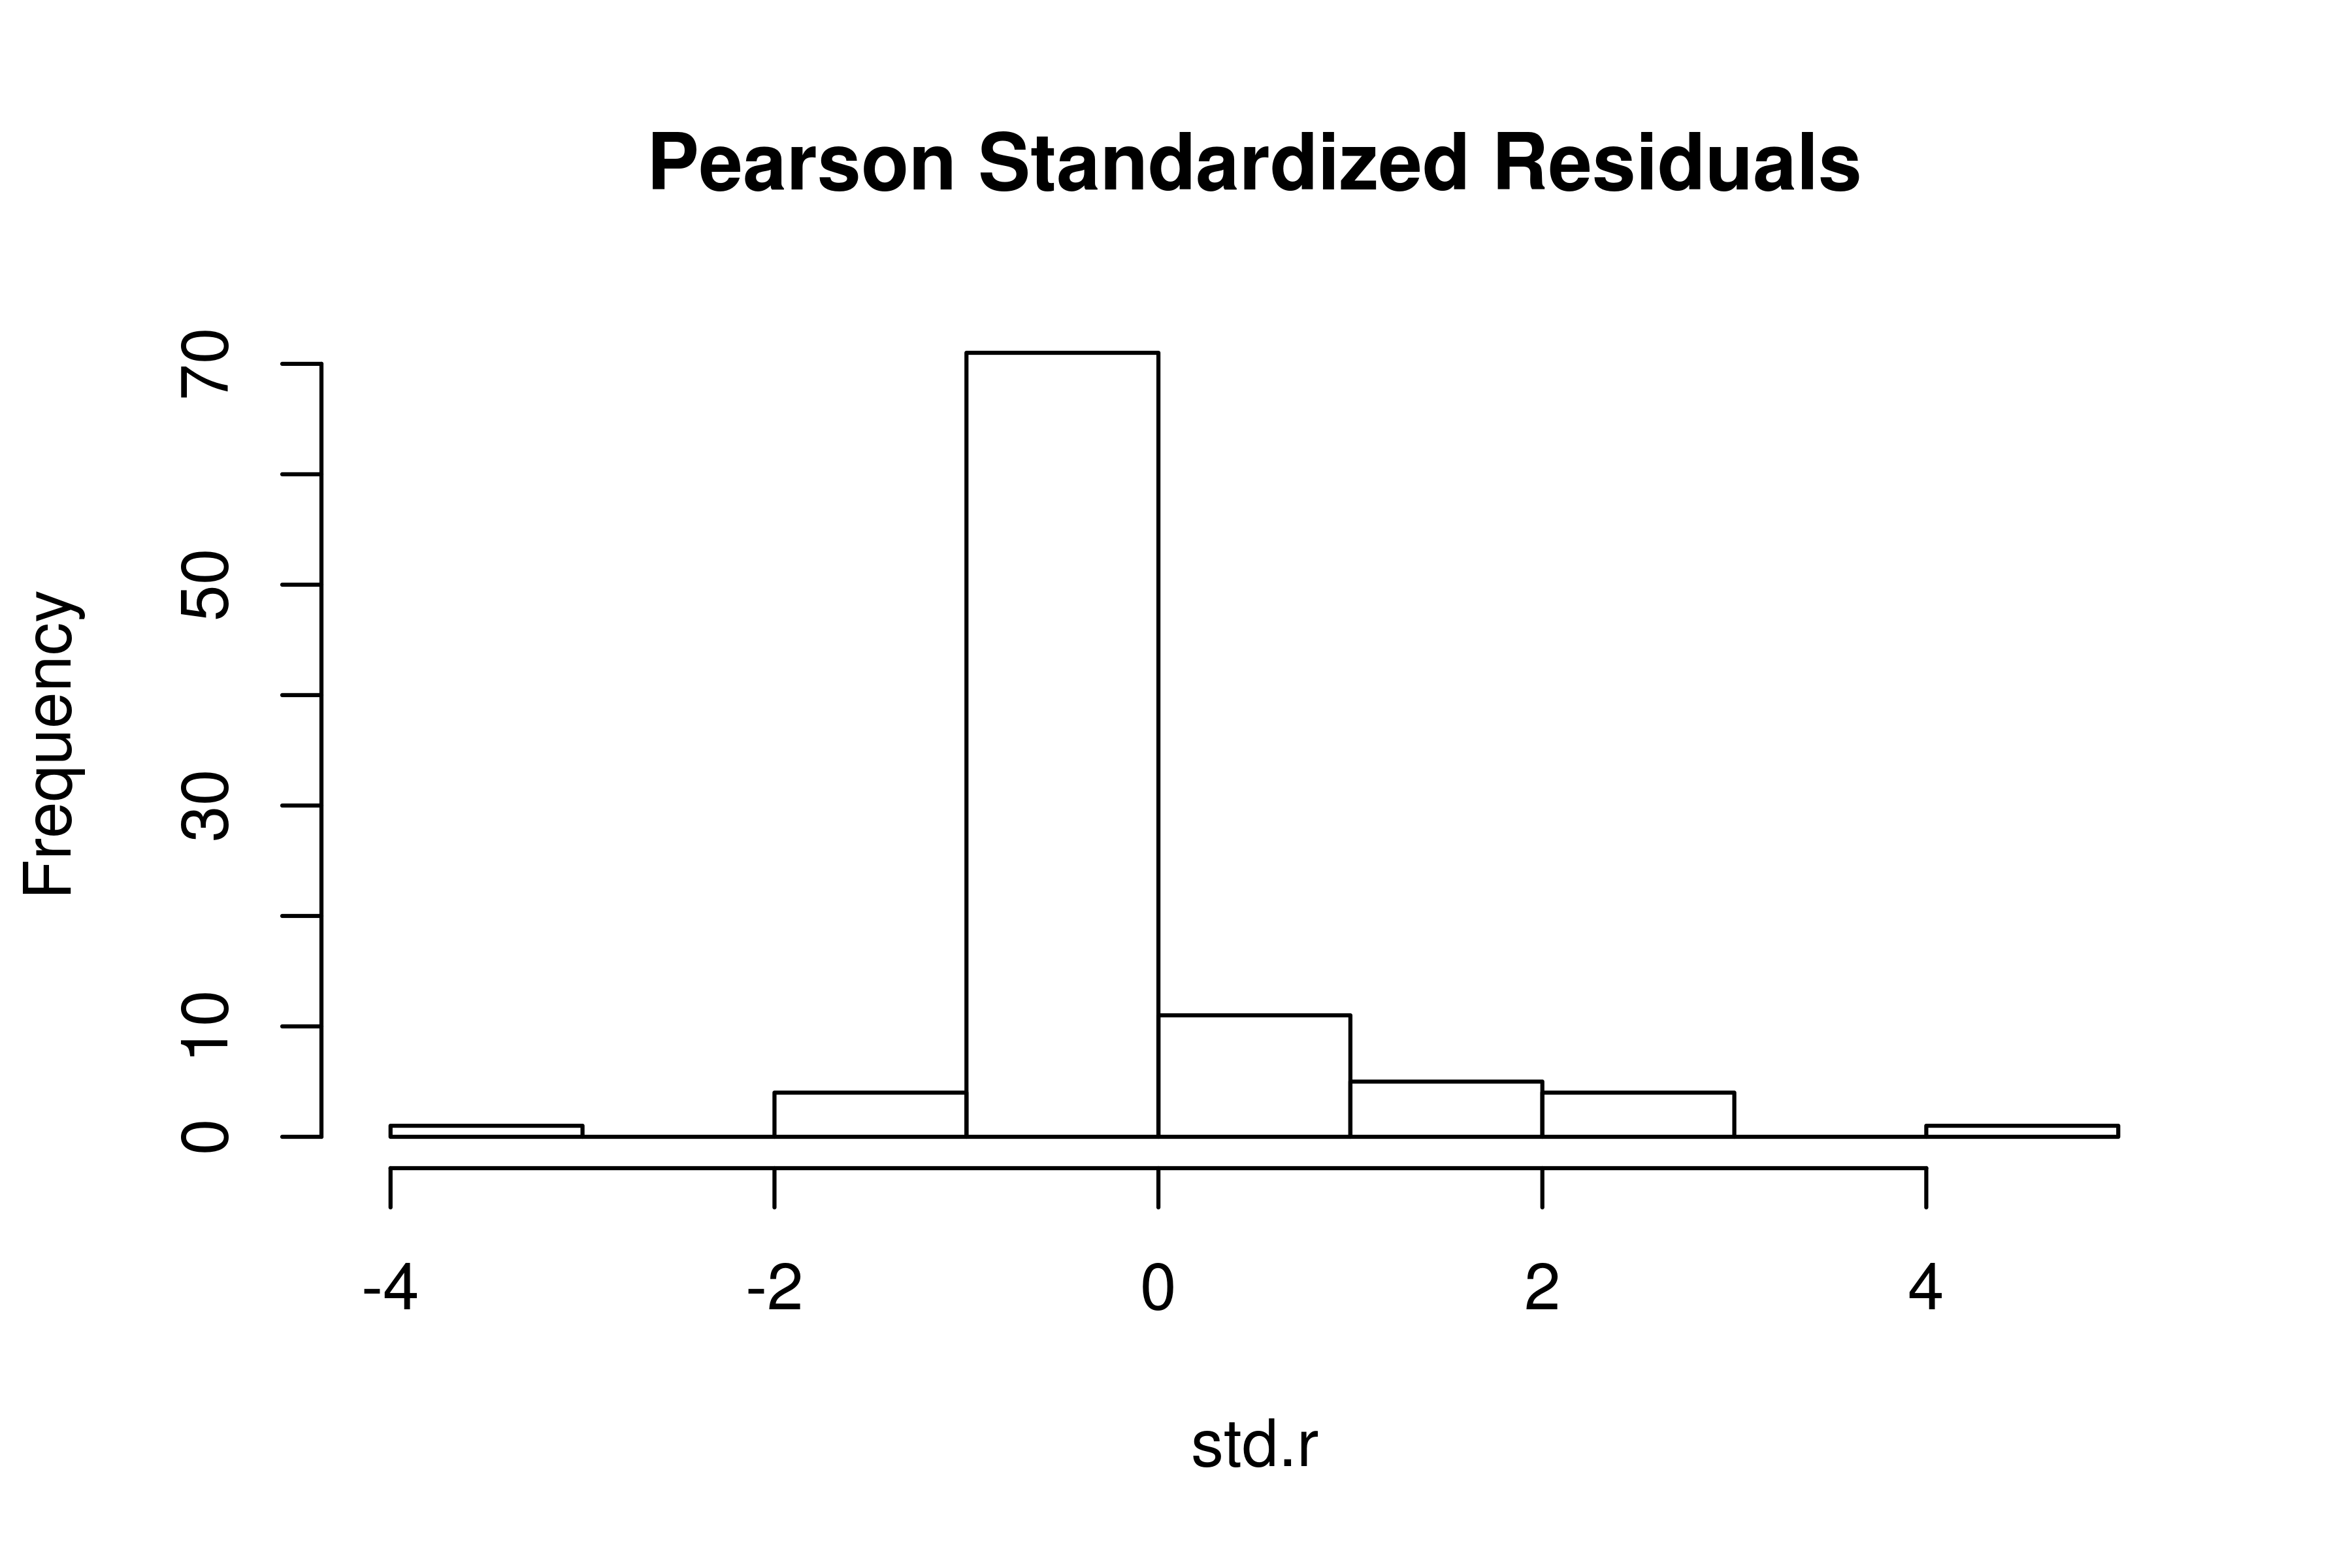
\includegraphics[width=0.6\textwidth,height=0.3\textheight]{pearson_std_e.png}	
	\caption{Plot of standardized residuals}
\end{figure}
Judging from the plot, we can conclude that the standardized residuals of pearson is approximately normally distributed. \par Besides, in general, $|r_{i}|>3$ can be an outlier. Therefore, there are several outliers in the dateset.\par
\subsubsection{ROC and AUC}
Since sensitivity and specificity rely on the cutoff value $\pi_{0}$, ROC and AUC are usually used as a better criteria to judge if a model fits well and how good the model is.\par
\begin{figure}[H]
	\centering
	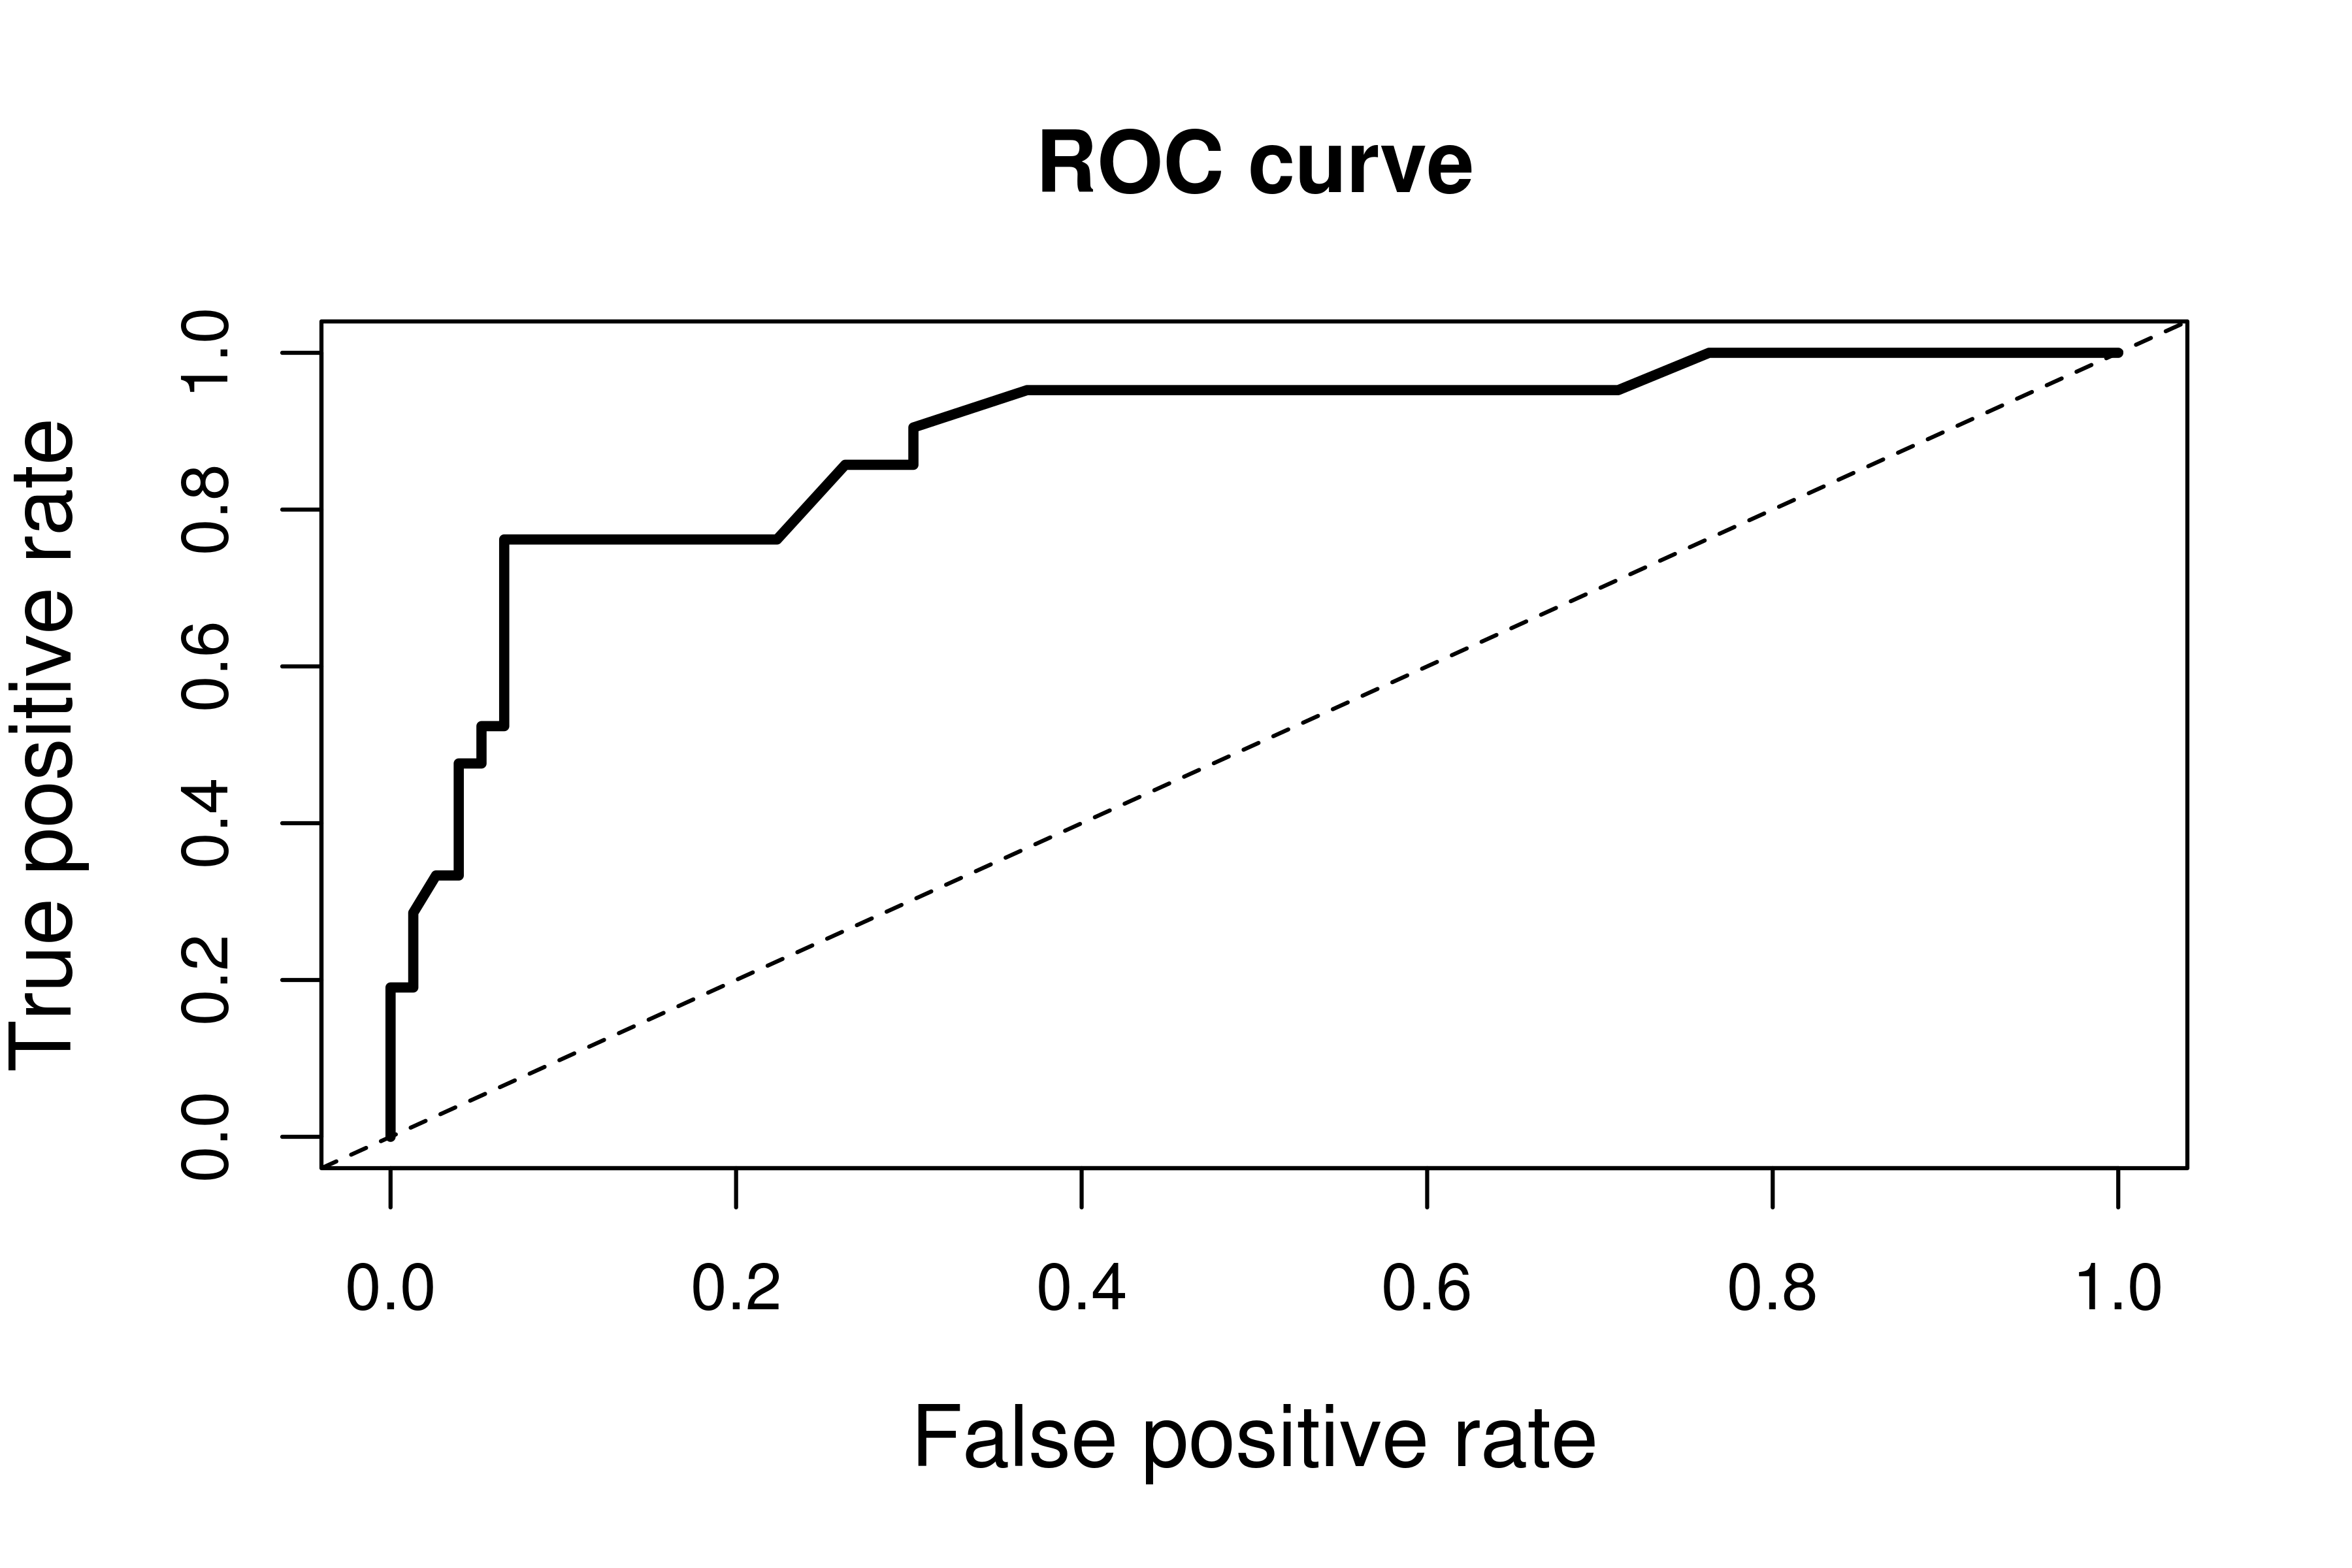
\includegraphics[width=0.6\textwidth,height=0.3\textheight]{auc.png}	
	\caption{ROC}
\end{figure}
AUC equals $0.8835$, $95\%$ CI for AUC is $[0.7977, 0.9693]$ and does not contain $0.5$. We can conclude that the model is very well fit.\par
\subsection{Remove Outliers}
We know that in logistic regression repeated rows may be diagnosed as influential points using leave-one-out measures like DfBeta and $\Delta\chi^2$. However, considering that there are 6 numeric explanatory variables in this dataset, it is almost impossible to have repeated rows. As a result, we treated all selected influential points as outliers. We removed 3 outliers, the ratio of which to the number of samples in the whole dataset is $3.09\%$, thus would not affect the dataset too much.\par
\begin{figure}[H]
	\centering
	\subfigure[Index plot of the change in the Pearson's test-statistics]{
		\begin{minipage}[b]{0.43\textwidth}
			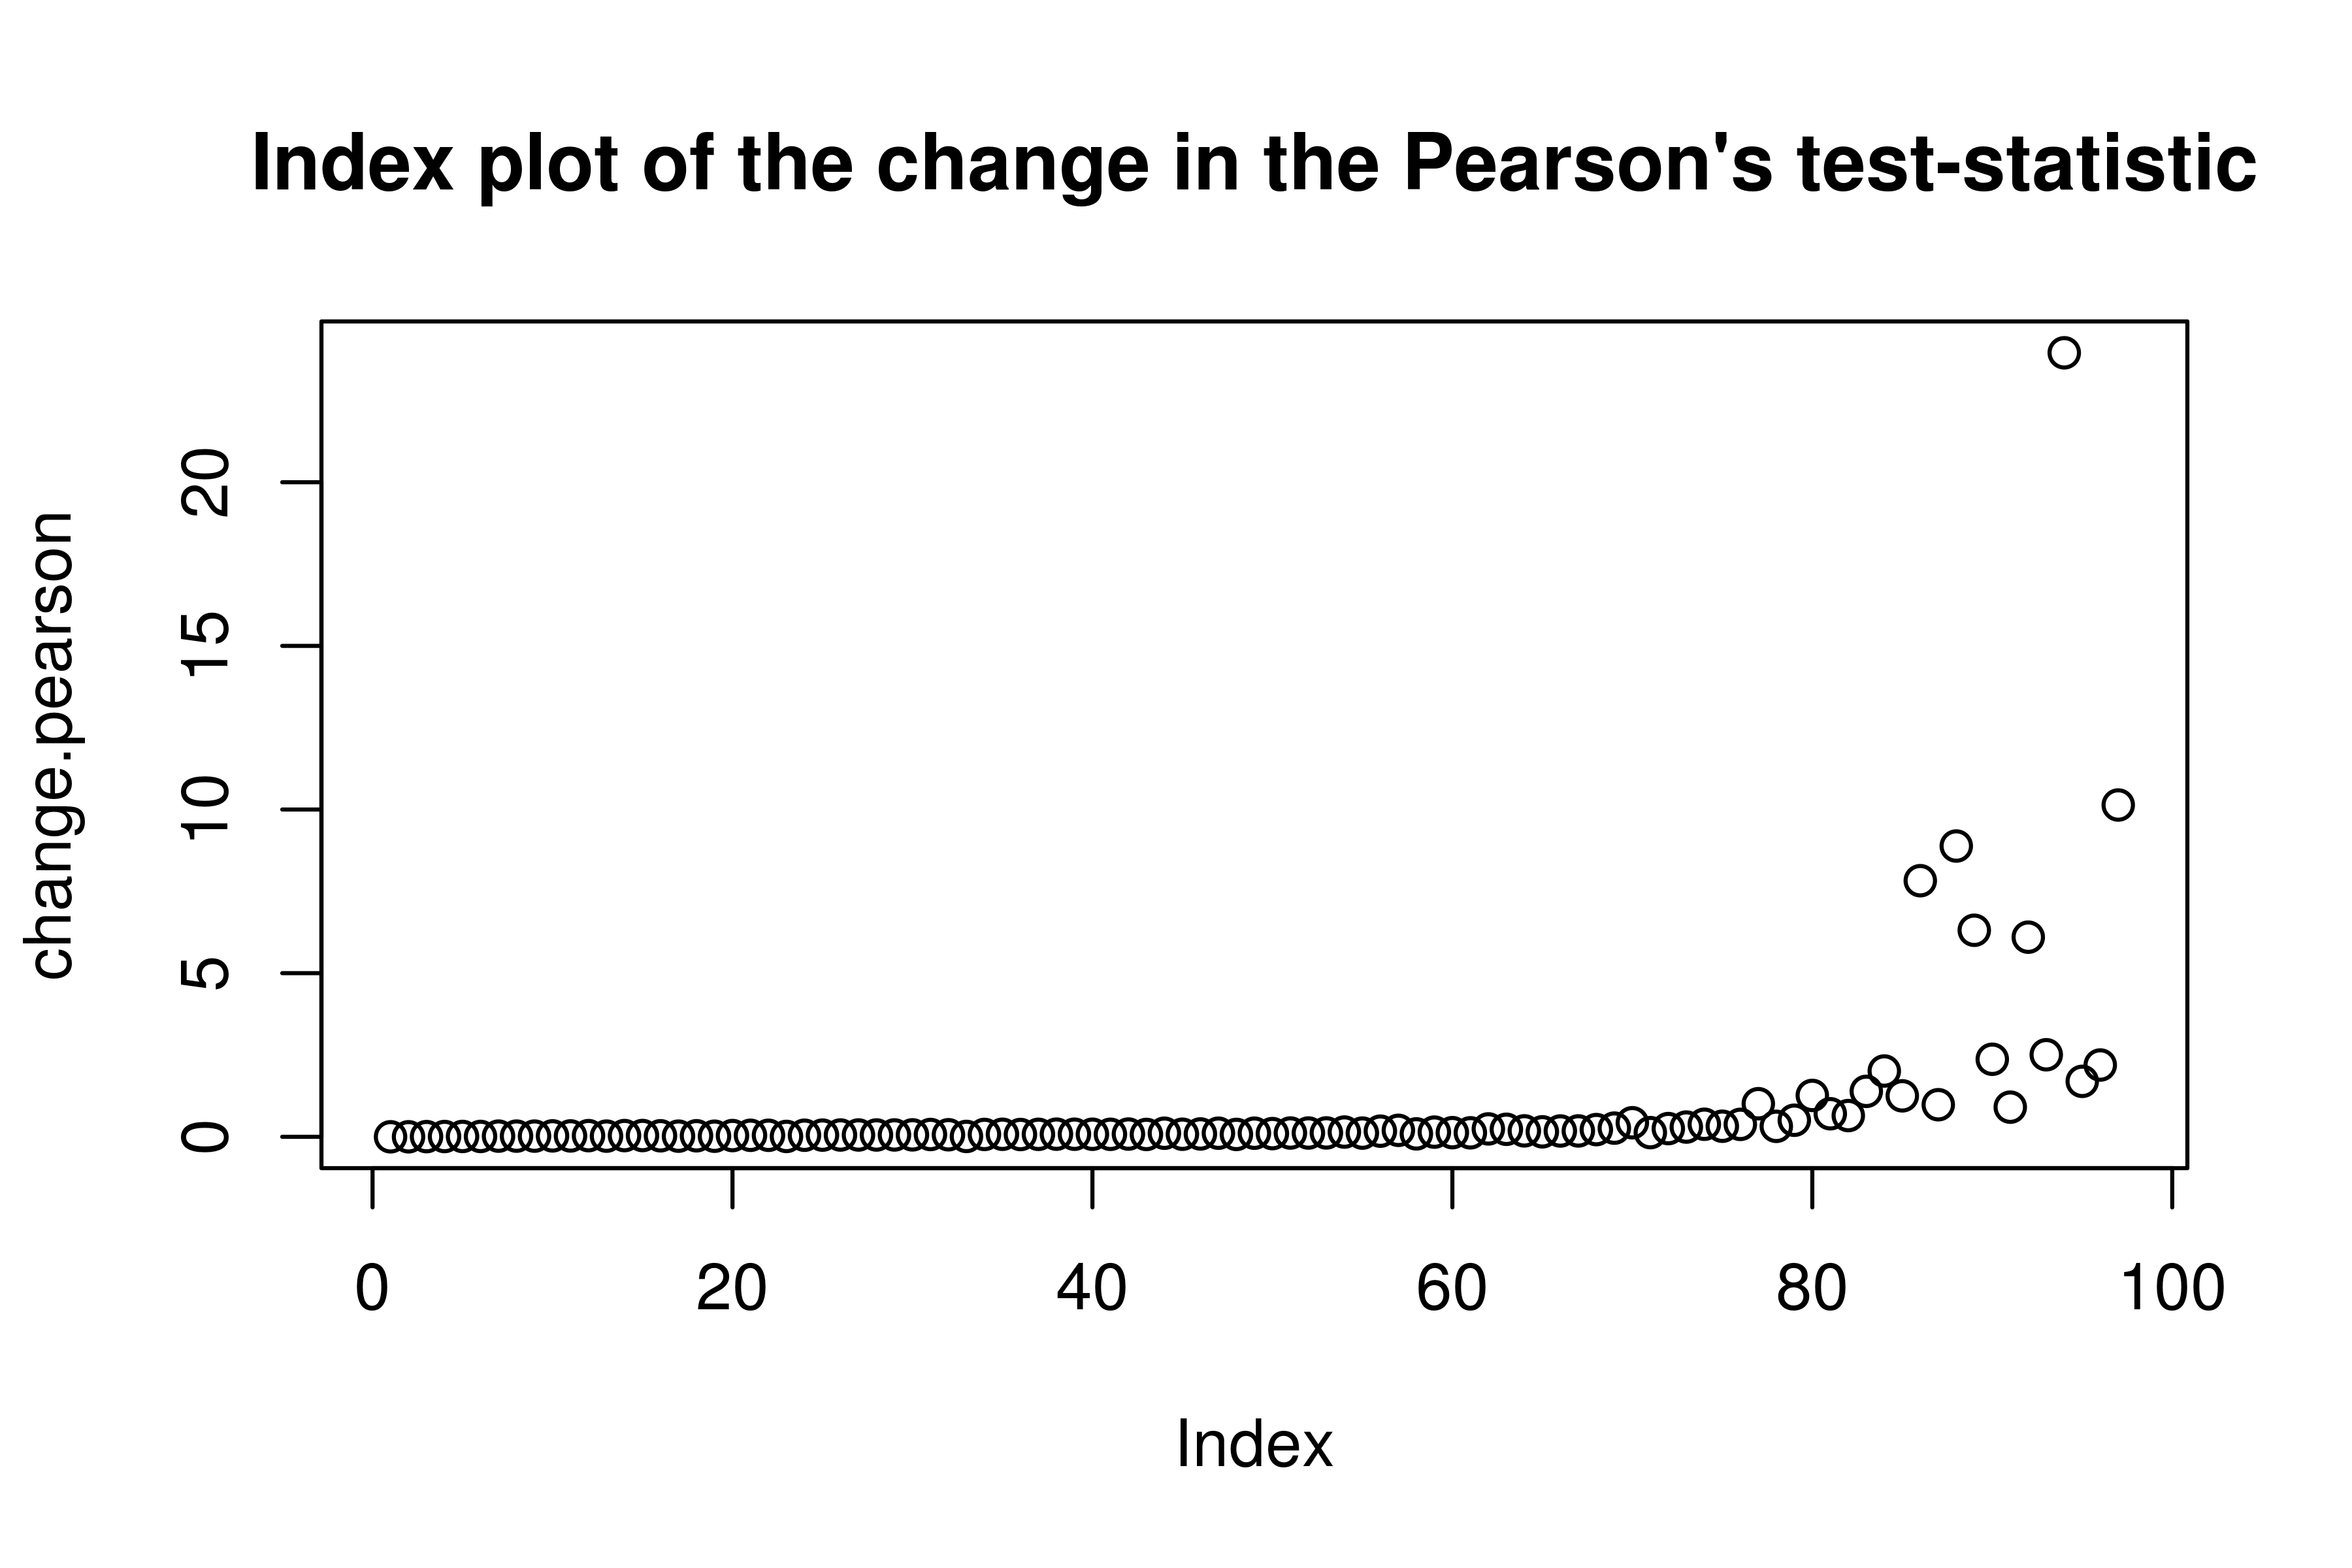
\includegraphics[width=1\textwidth,height=0.25\textheight]{dchisq.png} \\
		\end{minipage}
	}
	\subfigure[Index plot of the change in the Betas]{
		\begin{minipage}[b]{0.43\textwidth}
			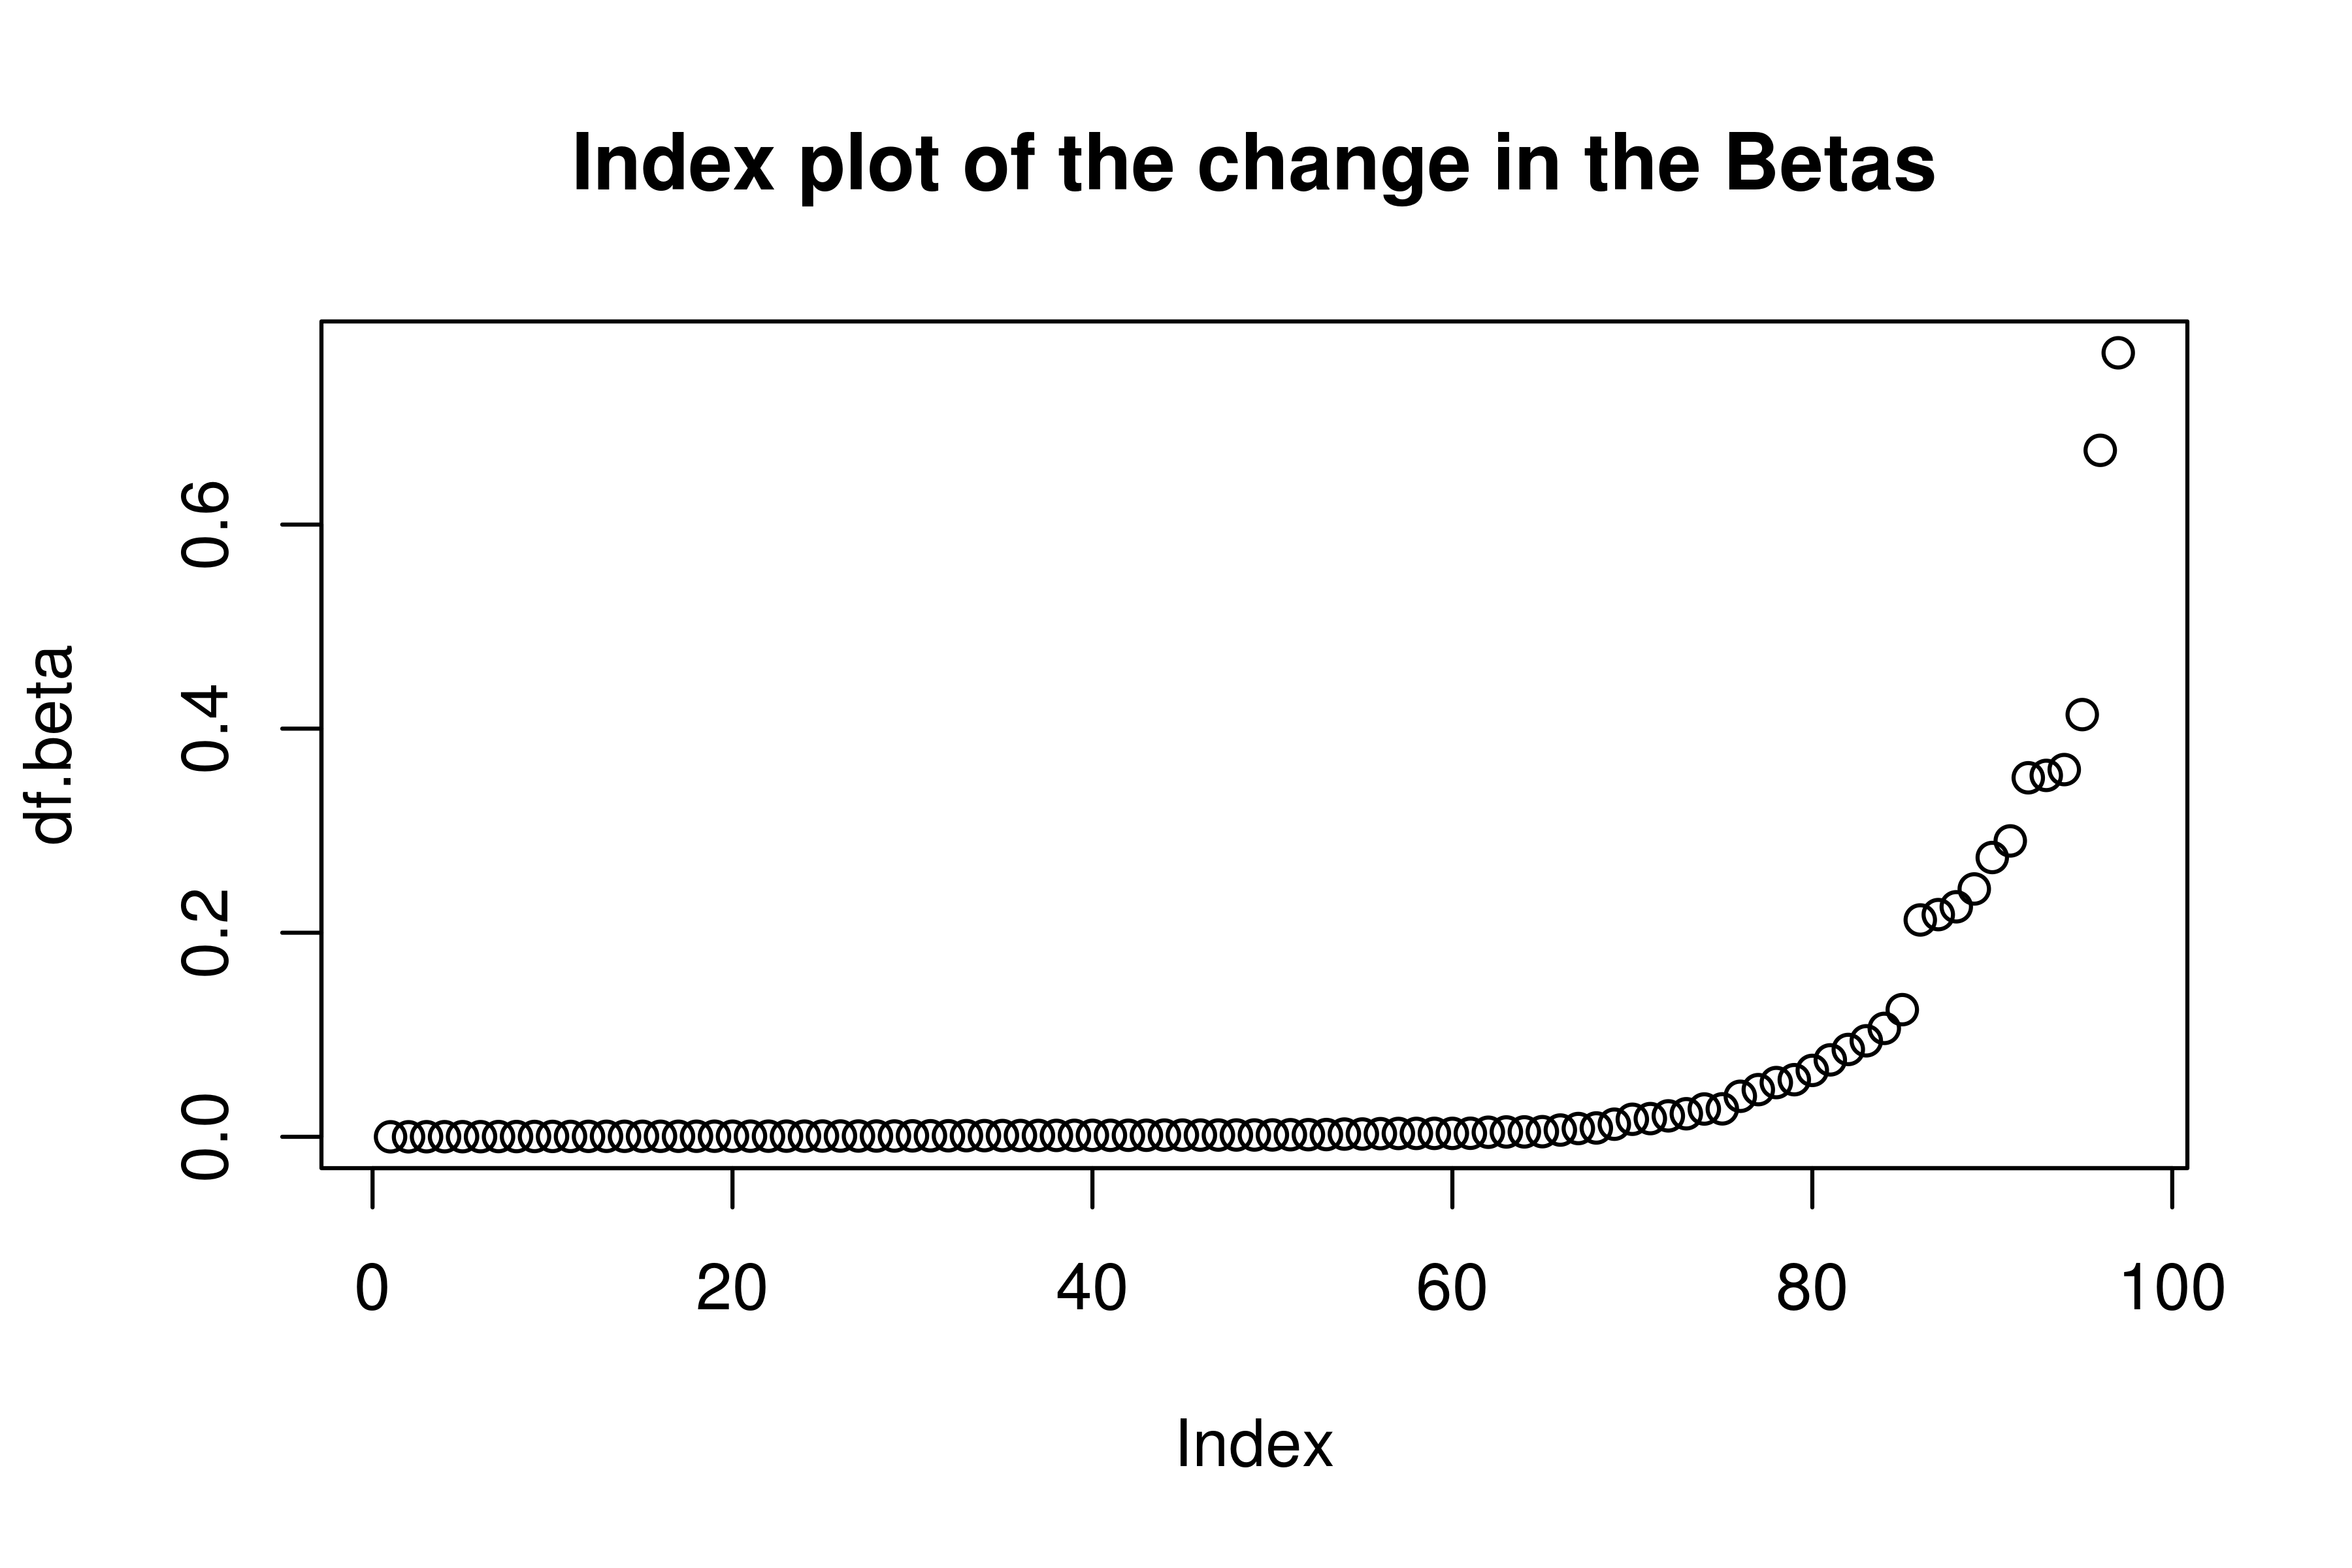
\includegraphics[width=1\textwidth,height=0.25\textheight]{dfbeta.png} \\
		\end{minipage}
	}
	\caption{Plots to identify outliers}
\end{figure}
\begin{table}[H]
	\centering
	\begin{tabular}{cc}
		\midrule[1.5pt]
		criteria&cutoff\\
		\hline 
		change.pearson&15\\
		df.beta&0.50\\
		\midrule[1.5pt]
	\end{tabular}
	\caption{Cutoff}
\end{table}
According to standardized residuals and Figure 3, outliers are as follows.\par
\begin{table}[H]
	\centering
	\begin{tabular}{ccccccccc}
		\midrule[1.5pt]
		index &Y  &X1   &X2   &X3  &X4   &X5   &X6    &X7\\
		\hline 
		41& 1&  9.974&  1.8589& 23.104& 60&  0& no-invasion&  0\\
		55& 1& 14.880& 23.3361& 33.784& 59&  0& no-invasion&  0\\
		91& 0& 56.261& 25.7903& 60.340& 68&  0& no-invasion&  0\\
		\midrule[1.5pt]
	\end{tabular}
	\caption{Outliers of the dataset}
\end{table}
\subsection{Final Model}
Finally, \texttt{psa}, \texttt{c.vol} and \texttt{age} are included in the final model. The logistic regression model is fitted using the dataset removed outliers.\par
\begin{equation}
\ln\left(\frac{\hat{\pi}}{1-\hat{\pi}}\right)= -13.5201+0.0648X_{1}+0.1285X_{2}+0.1428X_{4}  
\end{equation}
\begin{table}[H]
	\centering
	\begin{tabular}{cccc}
		\midrule[1.5pt]
		&$\hat{\beta}$&$\exp(\hat{\beta})$&Pr(>|z|)\\
		\hline 
		\texttt{Intercept} &-13.52014&1.3436$\times 10^{-6}$&0.0049\\ 
		\texttt{X1} &0.06481 &1.06695&0.0230\\ 
		\texttt{X2} &0.12850 &1.13712&0.0449\\
		\texttt{X4} &0.14279&1.15349&0.0376\\ 
		\midrule[1.5pt]
	\end{tabular}
	\caption{Coefficients of the final model}
\end{table}  
Interpretation of p-values for t-test of $\hat{\beta_{i}}$'s.\par
\begin{itemize}
	\item p-value for $\hat{\beta_{1}}$ : If the infomation on serum prostate-specific antigen level was dropped from the model, we would observe our data or more extreme with the probability of 0.0230.
	\item p-value for $\hat{\beta_{2}}$ : If the infomation on cancer volume was dropped from the model, we would observe our data or more extreme with the probability of 0.0449.
	\item p-value for $\hat{\beta_{3}}$ : If the infomation on age was dropped from the model, we would observe our data or more extreme with the probability of 0.0376.
\end{itemize}
\begin{table}[H]
	\centering
	\begin{tabular}{ccc}
		\midrule[1.5pt]
		&$2.5\%$&$97.5\%$\\
		\hline 
		\texttt{exp.X1}&1.0174 &1.1374\\
		\texttt{exp.X2}&1.0086 &1.3029\\
		\texttt{exp.X4}&1.0192 &1.3397\\
		\midrule[1.5pt]
	\end{tabular}
	\caption{$95\%$ Confidence Intervals for $\exp(\hat{\beta})$'s in the final model}
\end{table}


\subsubsection{Error Matrix}
We set the value of cutoff $\pi_{0}$ to $0.30$, and get the following matrix, with a sensitivity of 0.7895, a specificity of 0.9200 and an error-rate of 0.1064.
\begin{table}[H]
	\centering
	\begin{tabular}{ccc}
		\midrule[1.5pt]
		&$\hat{y}=0$&$\hat{y}=1$\\
		\hline 
		$y=0$& 69&  6\\
		$y=1$& 4&  15\\
		\midrule[1.5pt]
	\end{tabular}
	\caption{Error Matrix}
\end{table}

\subsubsection{Predictive Power}
\begin{equation}
\begin{aligned}
1-\frac{SSE}{SSTO}& = 1-\sum_{i=0}^{n}(y_{i}-\hat{\pi_{i}})^{2}/\sum_{i=0}^{n}(y_{i}-\bar{y})^{2}\\
&= 0.5069
\end{aligned}
\end{equation}
\par
When we use Logistic Regression  instead of $\bar{y}$ to predict the probability of a patient who is being assessed for prostate cancer, we can reduce the error by 50.69$\%$.\par
\subsection{Interpretation}
In this section, we are going to interpret $\hat{\beta_{i}}$'s and CI's of test-statistics in terms of the problem. (Note that p-values of test-statistics have already been interpreted in the context)\par
\subsubsection{$\hat{\beta_{i}}$'s}
\begin{itemize}
	\item $\exp(\hat{\beta_{0}})$: It is inappropriate to interpret $\hat{\beta_{0}}$, since 0 is not within the reasonable range for $X_{1}$, $X_{2}$ and $X_{4}$.
	\item $\exp(\hat{\beta_{1}})$: The odds of diagnosis with prostate cancer are multiplied by 1.0670 when serum prostate-specific antigen level increases by 1 mg/mL, holding all other variables constant.
	\item $\exp(\hat{\beta_{2}})$: The odds of diagnosis with prostate cancer are multiplied by 1.1371 when prostate cancer volume increases by 1 cc, holding all other variables constant.
	\item $\exp(\hat{\beta_{3}})$: The odds of diagnosis with prostate cancer are multiplied by 1.1535 when age of patient incrases by 1 year, holding all other variables constant.
\end{itemize}
\subsubsection{CI's for $\hat{\beta_{i}}$'s}
\begin{itemize}
	\item CI for $\exp(\hat{\beta_{1}})$: We are 95\% confident that the odds of diagnosis with prostate cancer tend to be multiplied by between 1.0174 and 1.1374 when serum prostate-specific antigen level increases by 1 mg/mL, holding all other variables constant.
	\item CI for $\exp(\hat{\beta_{2}})$: We are 95\% confident that the odds of diagnosis with prostate cancer tend to be multiplied by between 1.0086 and 1.3029 when prostate cancer volume increases by 1 cc, holding all other variables constant.
	\item CI for $\exp(\hat{\beta_{3}})$: We are 95\% confident that the odds of diagnosis with prostate cancer tend to be multiplied by between 1.01922 and 1.3397 when age of patient increases by 1 year, holding all other variables constant. 
\end{itemize}
\subsection{Predict}
We used our model to answer this question, ``Predict the probability of prostate cancer diagnosis for someone with 10 psa, 5 c.vol, age 67."\par
\begin{table}[htbp]
	\centering
	\begin{tabular}{cc}
		\midrule[1.5pt]
		Name&Result\\
		\hline 
		$\hat{\pi_{i}}$&0.0652\\
		$\hat{y}$&0\\
		\midrule[1.5pt]
	\end{tabular}
	\caption{Prediction}
\end{table}
The probability of prostate cancer diagnosis for someone with 10 psa, 5 c.vol, age 67 is 0.0652, and it is small enough for us to conclude that he would not be diagnosed with prostate cancer.\par
\subsection{Conclusion}
It is safe to conclude that the infomation on age of patient has the most significant effect on the prediction of prostate cancer diagnosis since the coefficient of $\exp(\hat{\beta_{i}})$ is the largest positive value.\par



\section{Task 2: ANOVA}
\subsection{Introduction}
In this task, we applied ANOVA to analyze the dataset of ``cows.csv" which contains the information from cows fed different types of grass.\par
Our goal is to build a model to tell whether there exist significant differences between groups. The full model is as follows and we did some improvement to make our model more efficient.
\begin{equation}
Y_{ij}=\mu_i+\varepsilon_{ij}
\end{equation}
A summary table is listed below to interpret these variables. 
\begin{table}[htbp]
	\centering
	\begin{tabular}{cccc}
		\midrule[1.5pt]
		Name& Variable &Variable Kind  & Units\\
		\hline
		\texttt{Weight}&$Y$ & Response  & kg\\
		\texttt{Grass} &$X$& Catogorical  & A/B/C  \\
		\midrule[1.5pt]
	\end{tabular}
	\caption{A summary table for variables }
\end{table}
\subsection{Data Preparation}
\subsubsection{Summary Table}
Some useful statistics give us a brief review of basic information on our dataset. As shown in the table below, it is apparent that differences exist between varied categories.
\begin{table}[H]
	\centering
	\begin{tabular}{cccc}
		\midrule[1.5pt]	
		&A &B &C\\
		\hline
		Means&200.0&250.0&294.2\\
		Std. Dev&22.46&20.45&40.44\\			Sample Size &12&12&12\\
		\midrule[1.5pt]
	\end{tabular}
	\caption{Summary Table for data}
\end{table}
\subsubsection{Visualizing the Data}
By visualizing the data, it is obvious that the mean weight varies from group to group , which suggests the factor that different types of grass the cows were fed have a significant effect on the weight of cows.\par
From the grouped boxplot, we are convinced that there is no obvious outliers in our dataset.
\begin{figure}[H]
	\centering
	\subfigure[Mean of different groups]{
		\begin{minipage}[b]{0.43\textwidth}
			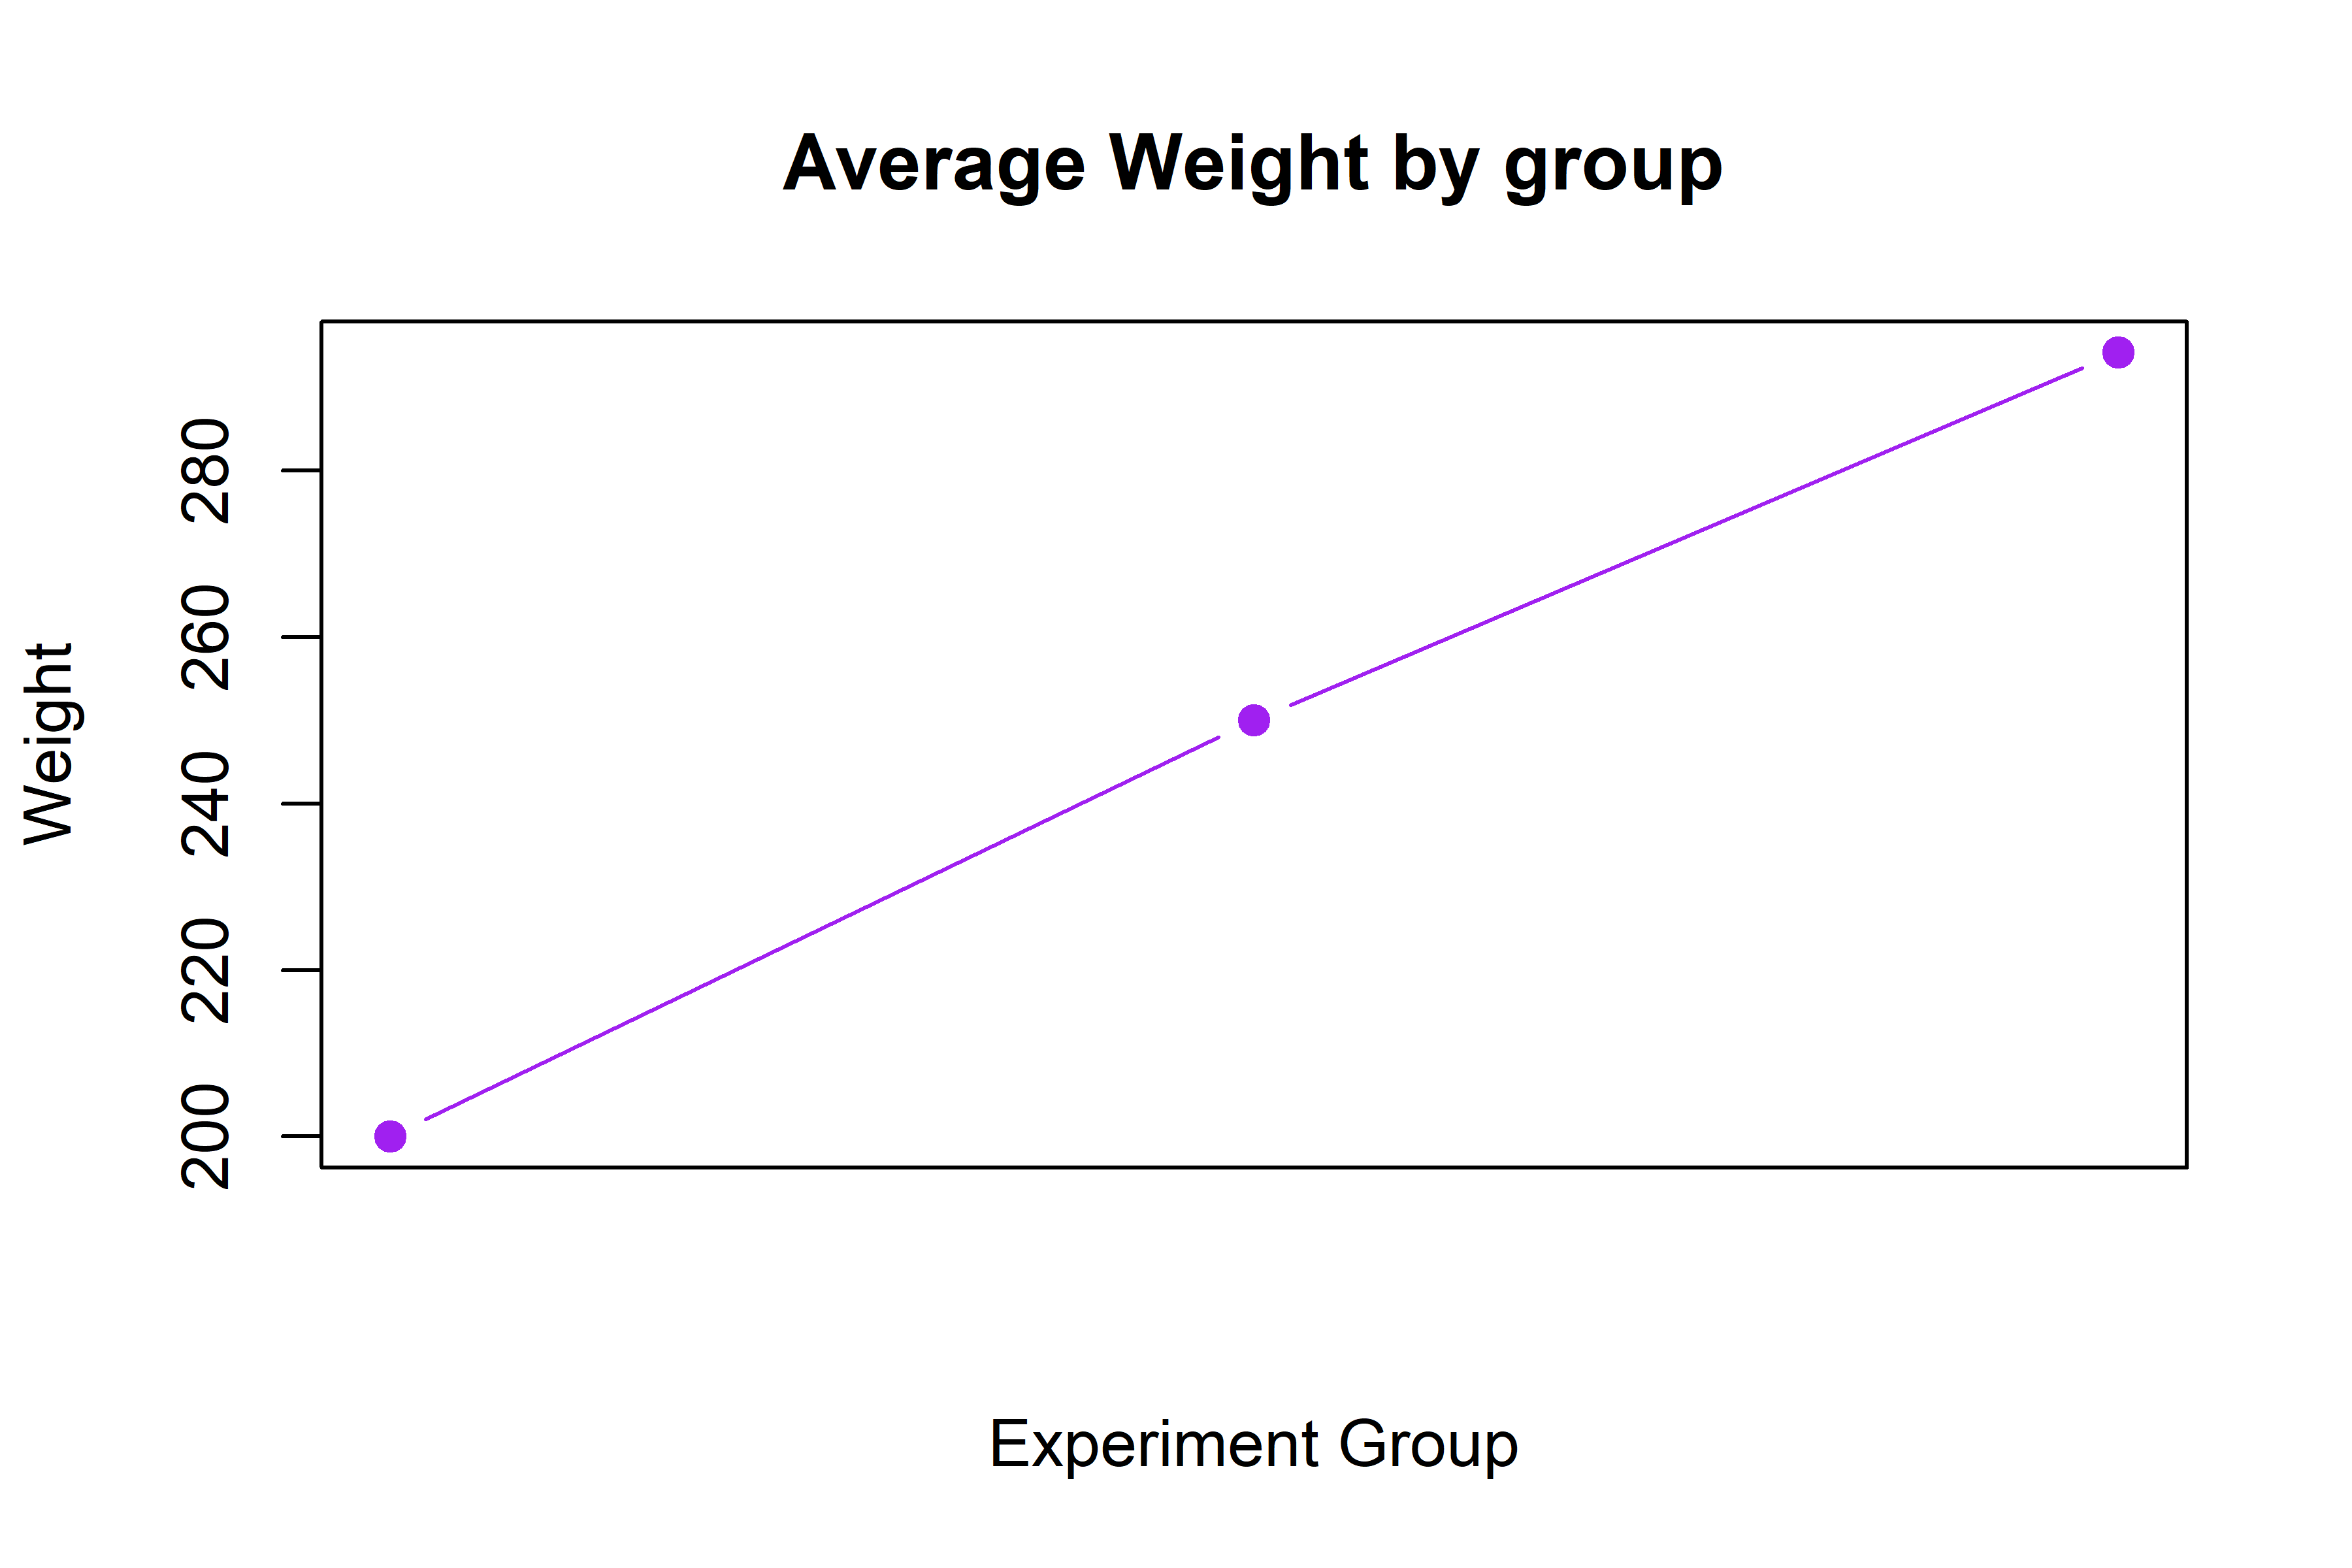
\includegraphics[width=1\textwidth,height=0.25\textheight]{1.png} \\
		\end{minipage}
	}
	\subfigure[Boxplot of weight vs Grass]{
		\begin{minipage}[b]{0.43\textwidth}
			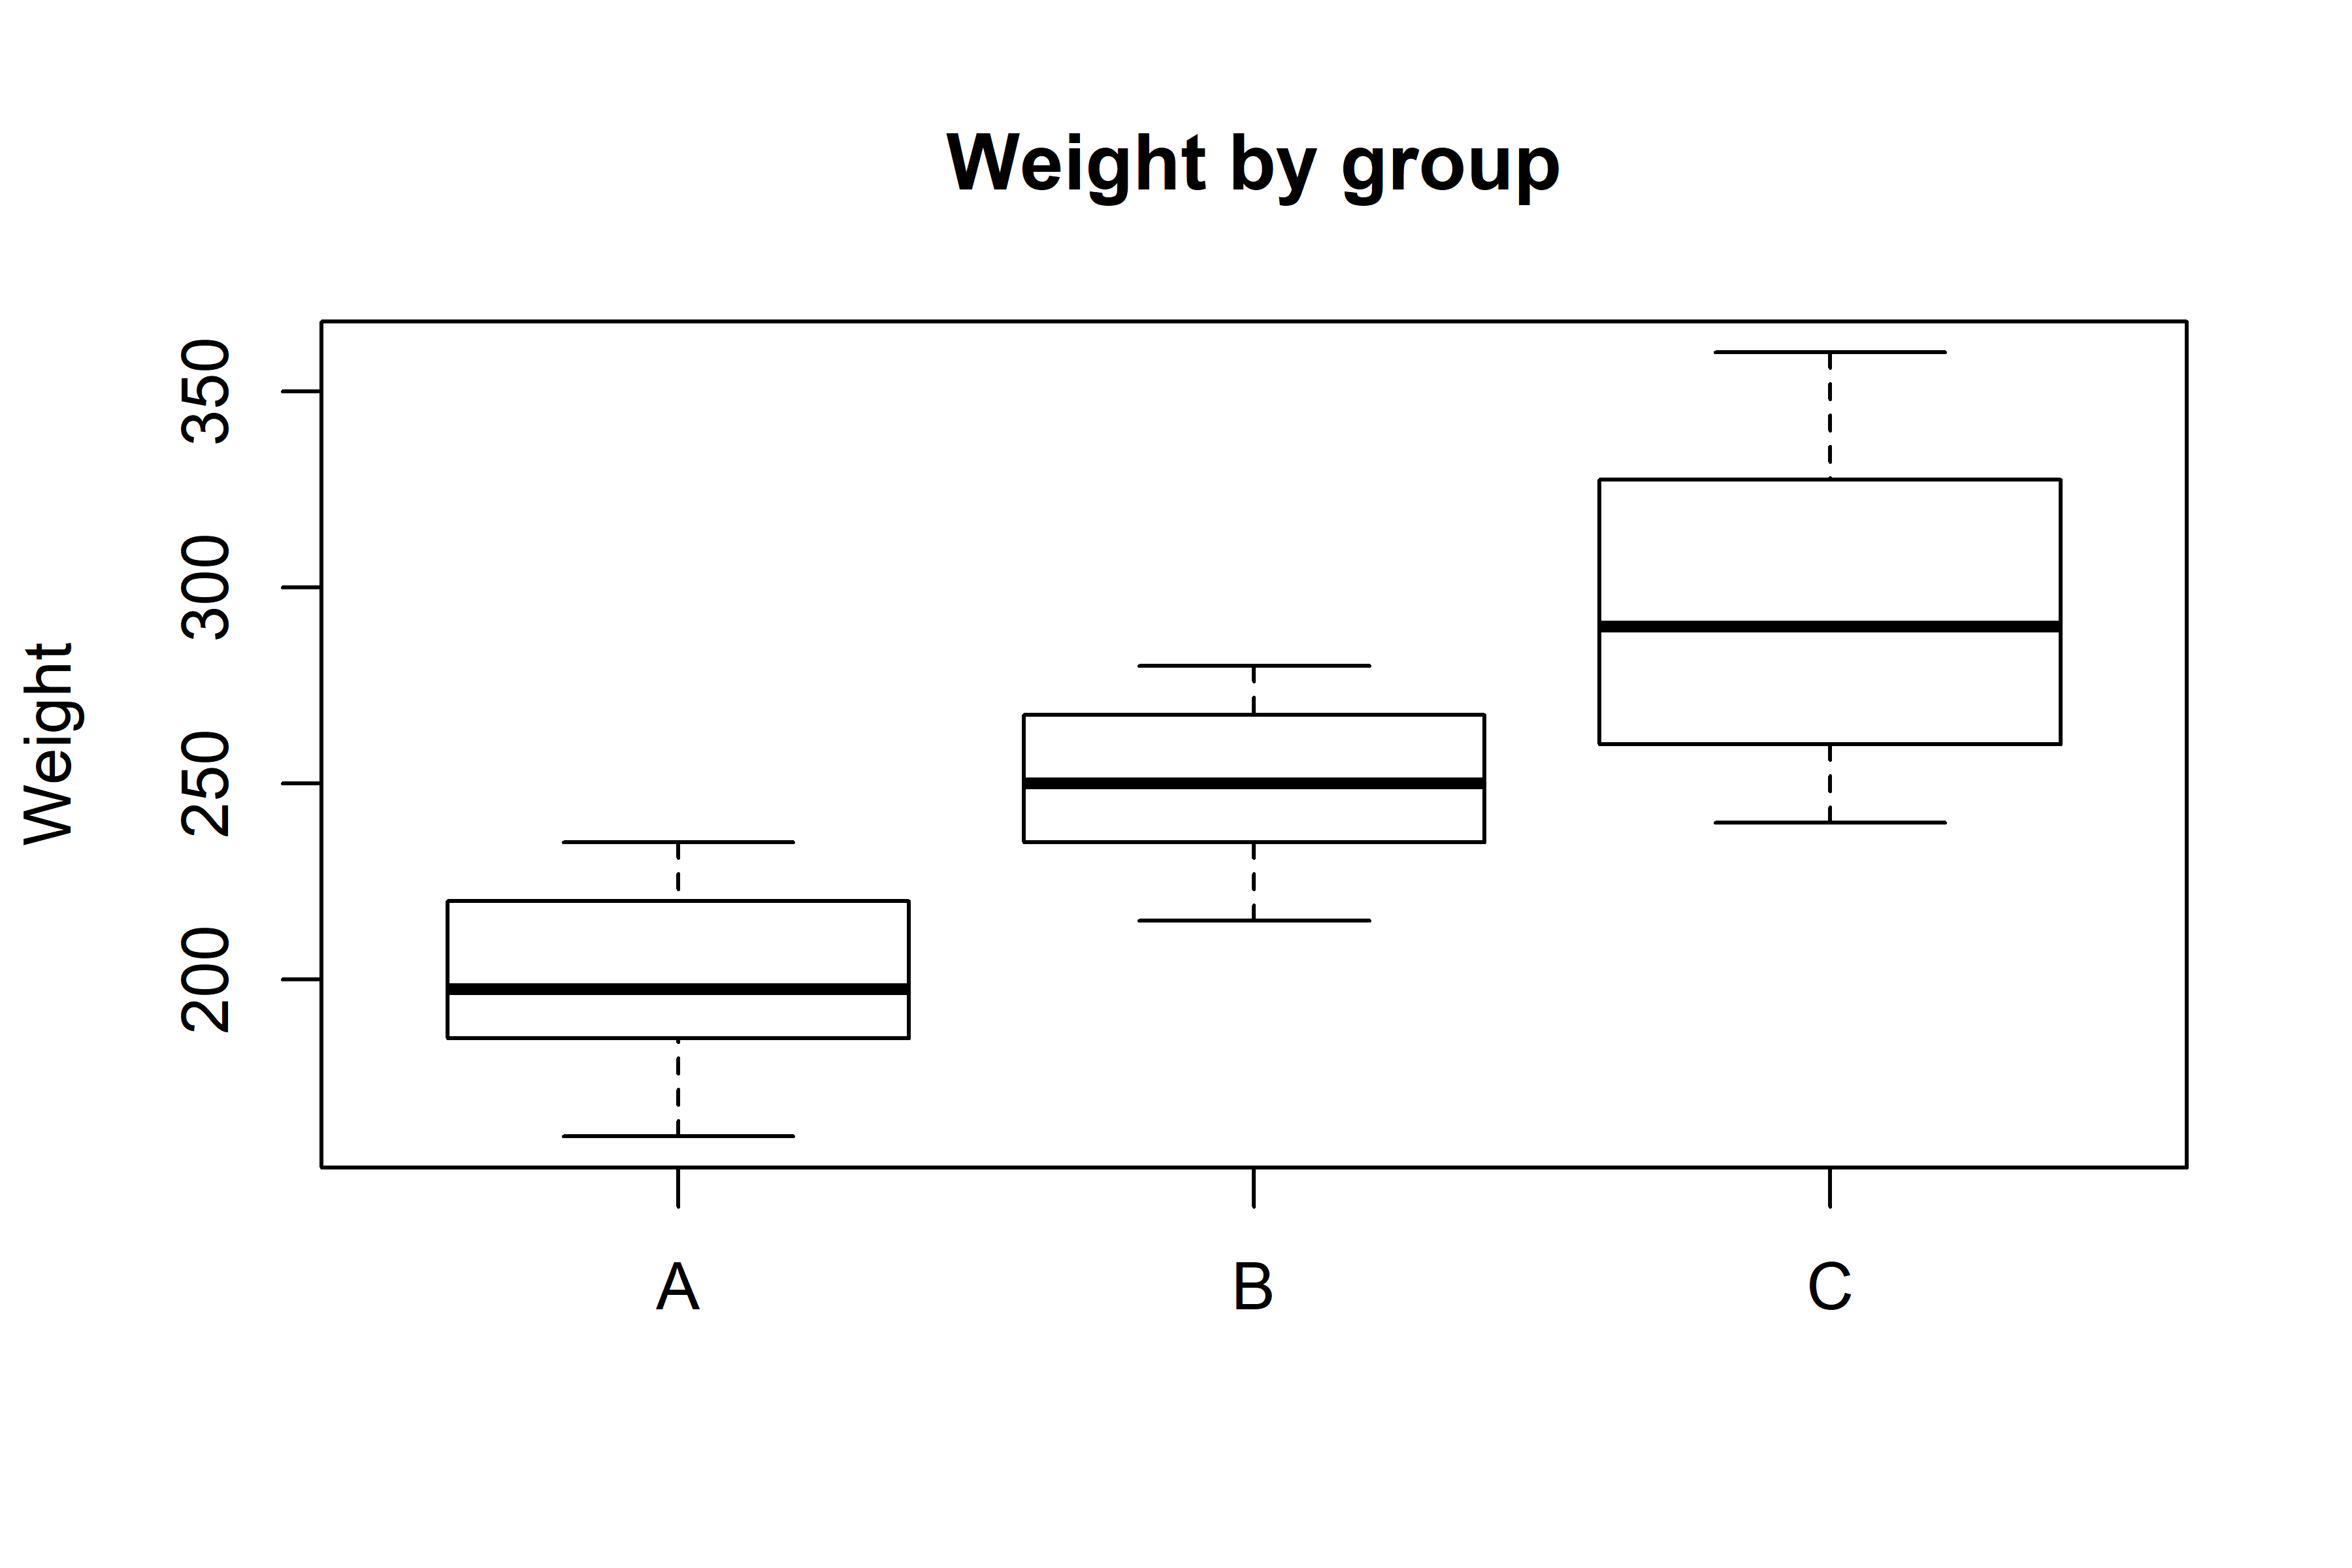
\includegraphics[width=1\textwidth,height=0.25\textheight]{2.png} \\
		\end{minipage}
	}
	\caption{Review of the dataset}
\end{figure}
\subsection{Simple one-way ANOVA}
\subsubsection{F-test}
We first use F-test to find whether type of grass is an important factor in the model.\par 
\begin{itemize}
	\item $H_0$: $\mu_A=\mu_B=\mu_C$. 
	\item $H_A$: Not all $\mu_i ( i=A,B,C ) $ are equal.
\end{itemize}
\par
According to R, the p-value for F-tset is almost 0. So we reject $H_0$ and conclude that the Grass group has a significant effect on cows' weight.\par 
Interpret the p-value of F-test above.
\begin{itemize}
	\item It means that if $\mu_A=\mu_B=\mu_C$ was true (types of grass had no significant difference on the weight of cows), we would observe our data or more exteme with the probability of almost 0\%.
\end{itemize}
\subsubsection{ANOVA Table}
\begin{table}[H]
	\centering
	\begin{tabular}{cccc}
		\midrule[1.5pt]	
		&difference &95 \% C.I. &p-value\\
		\hline
		$\mu_A-\mu_B$&-50.00&[-80.07,-19.93]&0.00058\\
		$\mu_A-\mu_C$&-94.17&[-124.2,-64.10]&0\\		 $\mu_B-\mu_{C}$&-44.17&[-74.24,-14.10]&0.002314\\
		\midrule[1.5pt]
	\end{tabular}
	\caption{ANOVA table for the data}
\end{table}
The C.I.'s based on Bonferroni does not contain 0 which means there exists significant difference between different groups.\par 
Interpretation  for p-values of F-test.
\begin{itemize}
	\item p-value for $\mu_A-\mu_B$: If there was no significant difference between the mean weight of cows fed grass A and grass B, we would observe our data or more extreme with the probability of 0.00058.
	\item p-value for $\mu_A-\mu_C$: If there was no significant difference between the mean weight of cows fed grass A and grass C, we would observe our data or more extreme with the probability of 0.
	\item p-value for $\mu_B-\mu_C$: If there was no significant difference between the mean weight of cows fed grass B and grass C, we would observe our data or more extreme with the probability of 0.002314.
\end{itemize}
\par
Interpret $\mu_i-\mu_j$ and the CI's for $\mu_i-\mu_j$.
\begin{itemize}
	\item $\mu_A-\mu_B$: The estimated weight gain (kg) in the cows fed grass A is 50.00kg smaller than the cows fed grass B.
	\item $\mu_A-\mu_C$: The The estimated weight gain (kg) in the cows fed grass A is 94.17kg smaller than the cows fed grass C.
	\item $\mu_B-\mu_C$: The The estimated weight gain (kg) in the cows fed grass B is 44.17kg smaller than the cows fed grass C.
\end{itemize}
\begin{itemize}
	\item CI for $\mu_A-\mu_B$: We are 95\% confident that weight gain (kg) in the cows fed grass A is smaller than the cows fed grass B by between 19.93kg and 80.07kg.
	\item CI for $\mu_A-\mu_C$: We are 95\% confident that weight gain (kg) in the cows fed grass A is smaller than the cows fed grass C by between 64.10kg and 124.2kg.
	\item CI for $\mu_B-\mu_C$: We are 95\% confident that weight gain (kg) in the cows fed grass B is smaller than the cows fed grass C by between 14.10kg and 74.24kg.
\end{itemize}
\subsection{Diagnostics for the model}
\subsubsection{Independence of $Y$}
\begin{figure}[H]
\centering
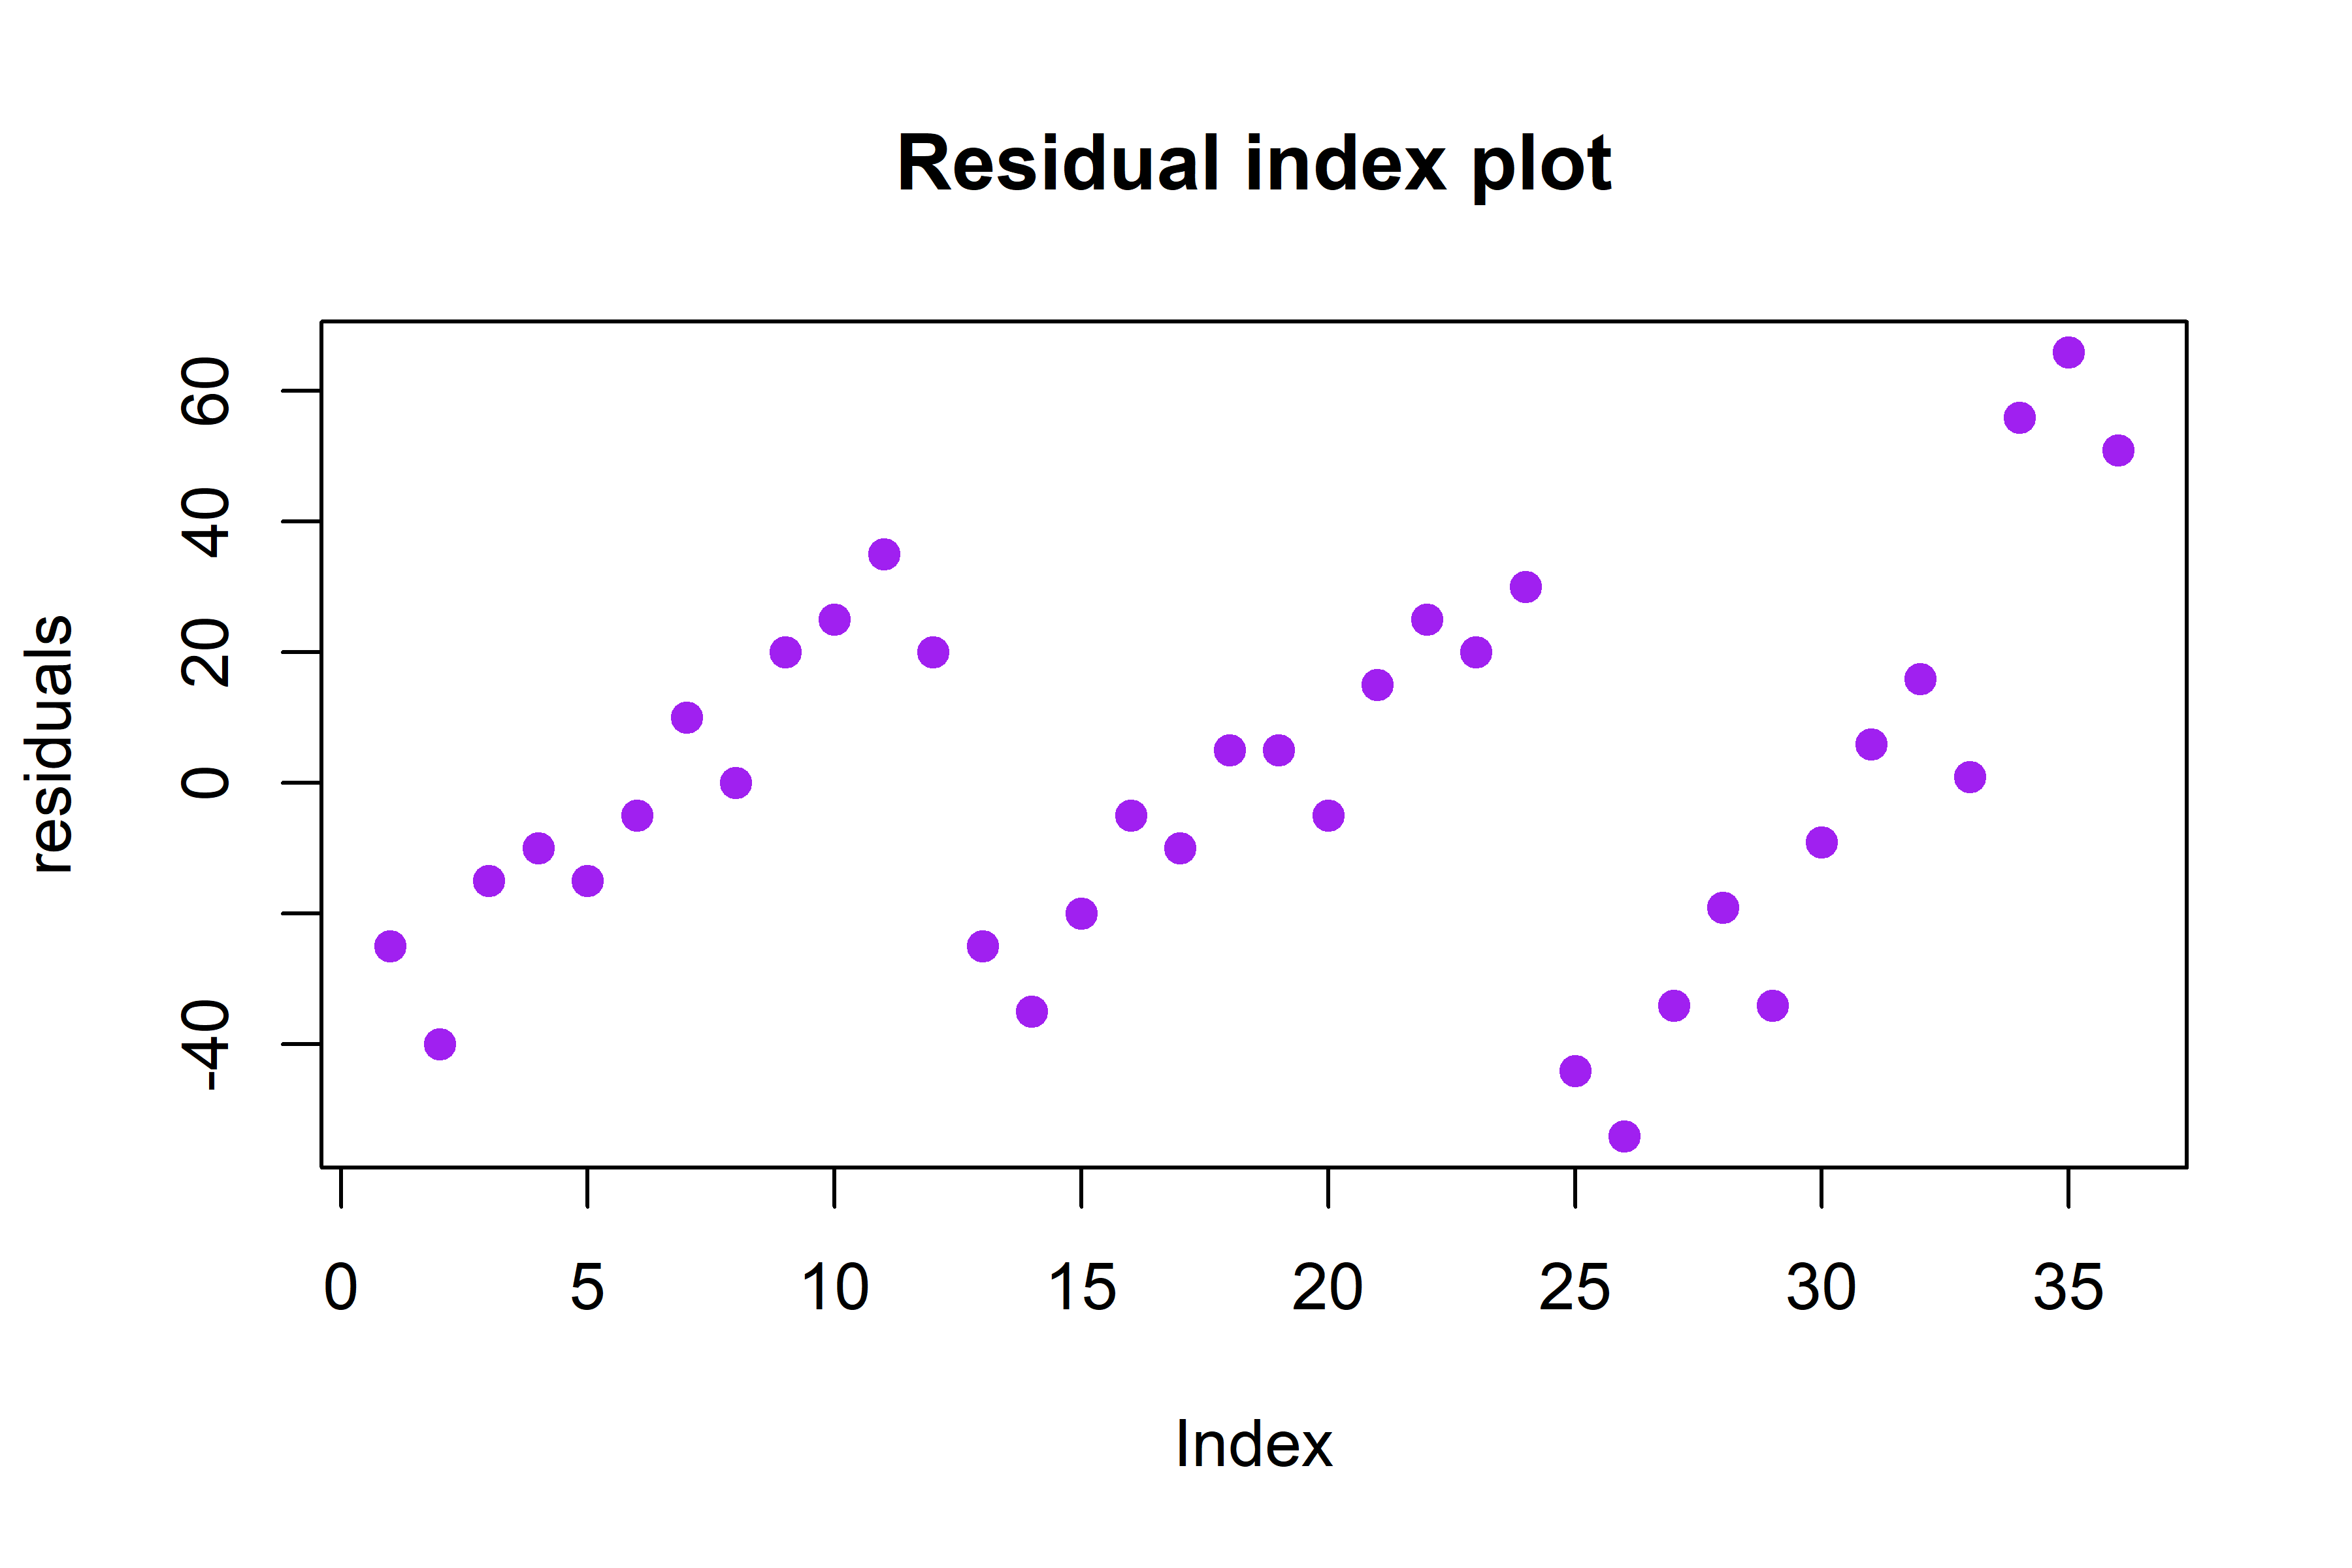
\includegraphics[width=0.6\textwidth,height=0.3\textheight]{3.png}	
\end{figure}
Index is just a subjective order of samples in the dataset, points on the plot can be randomly shuffled. Since there is no apparent pattern along the vertical axis, we can conclude that each sample is independently selected.
\subsubsection{Normality of errors}
We used Shapiro-Wilks test for error normality. According to R, the p-value is 0.8852. So we fail to reject the null hypothesis and conclude that the errors are normally distributed.\par  
Interpret p-value of the shapiro test .
\begin{itemize}
	\item If the errors were normally distributed, we would observe the data or more extreme 88.52\% of the time.
\end{itemize}
\par
Secondly, based on the Normal QQ Plot and the distribution of the residuals, we are convinced that the errors are normal.
\begin{figure}[H]
	\centering
	\subfigure[Residual Distribution Plot]{
		\begin{minipage}[b]{0.43\textwidth}
			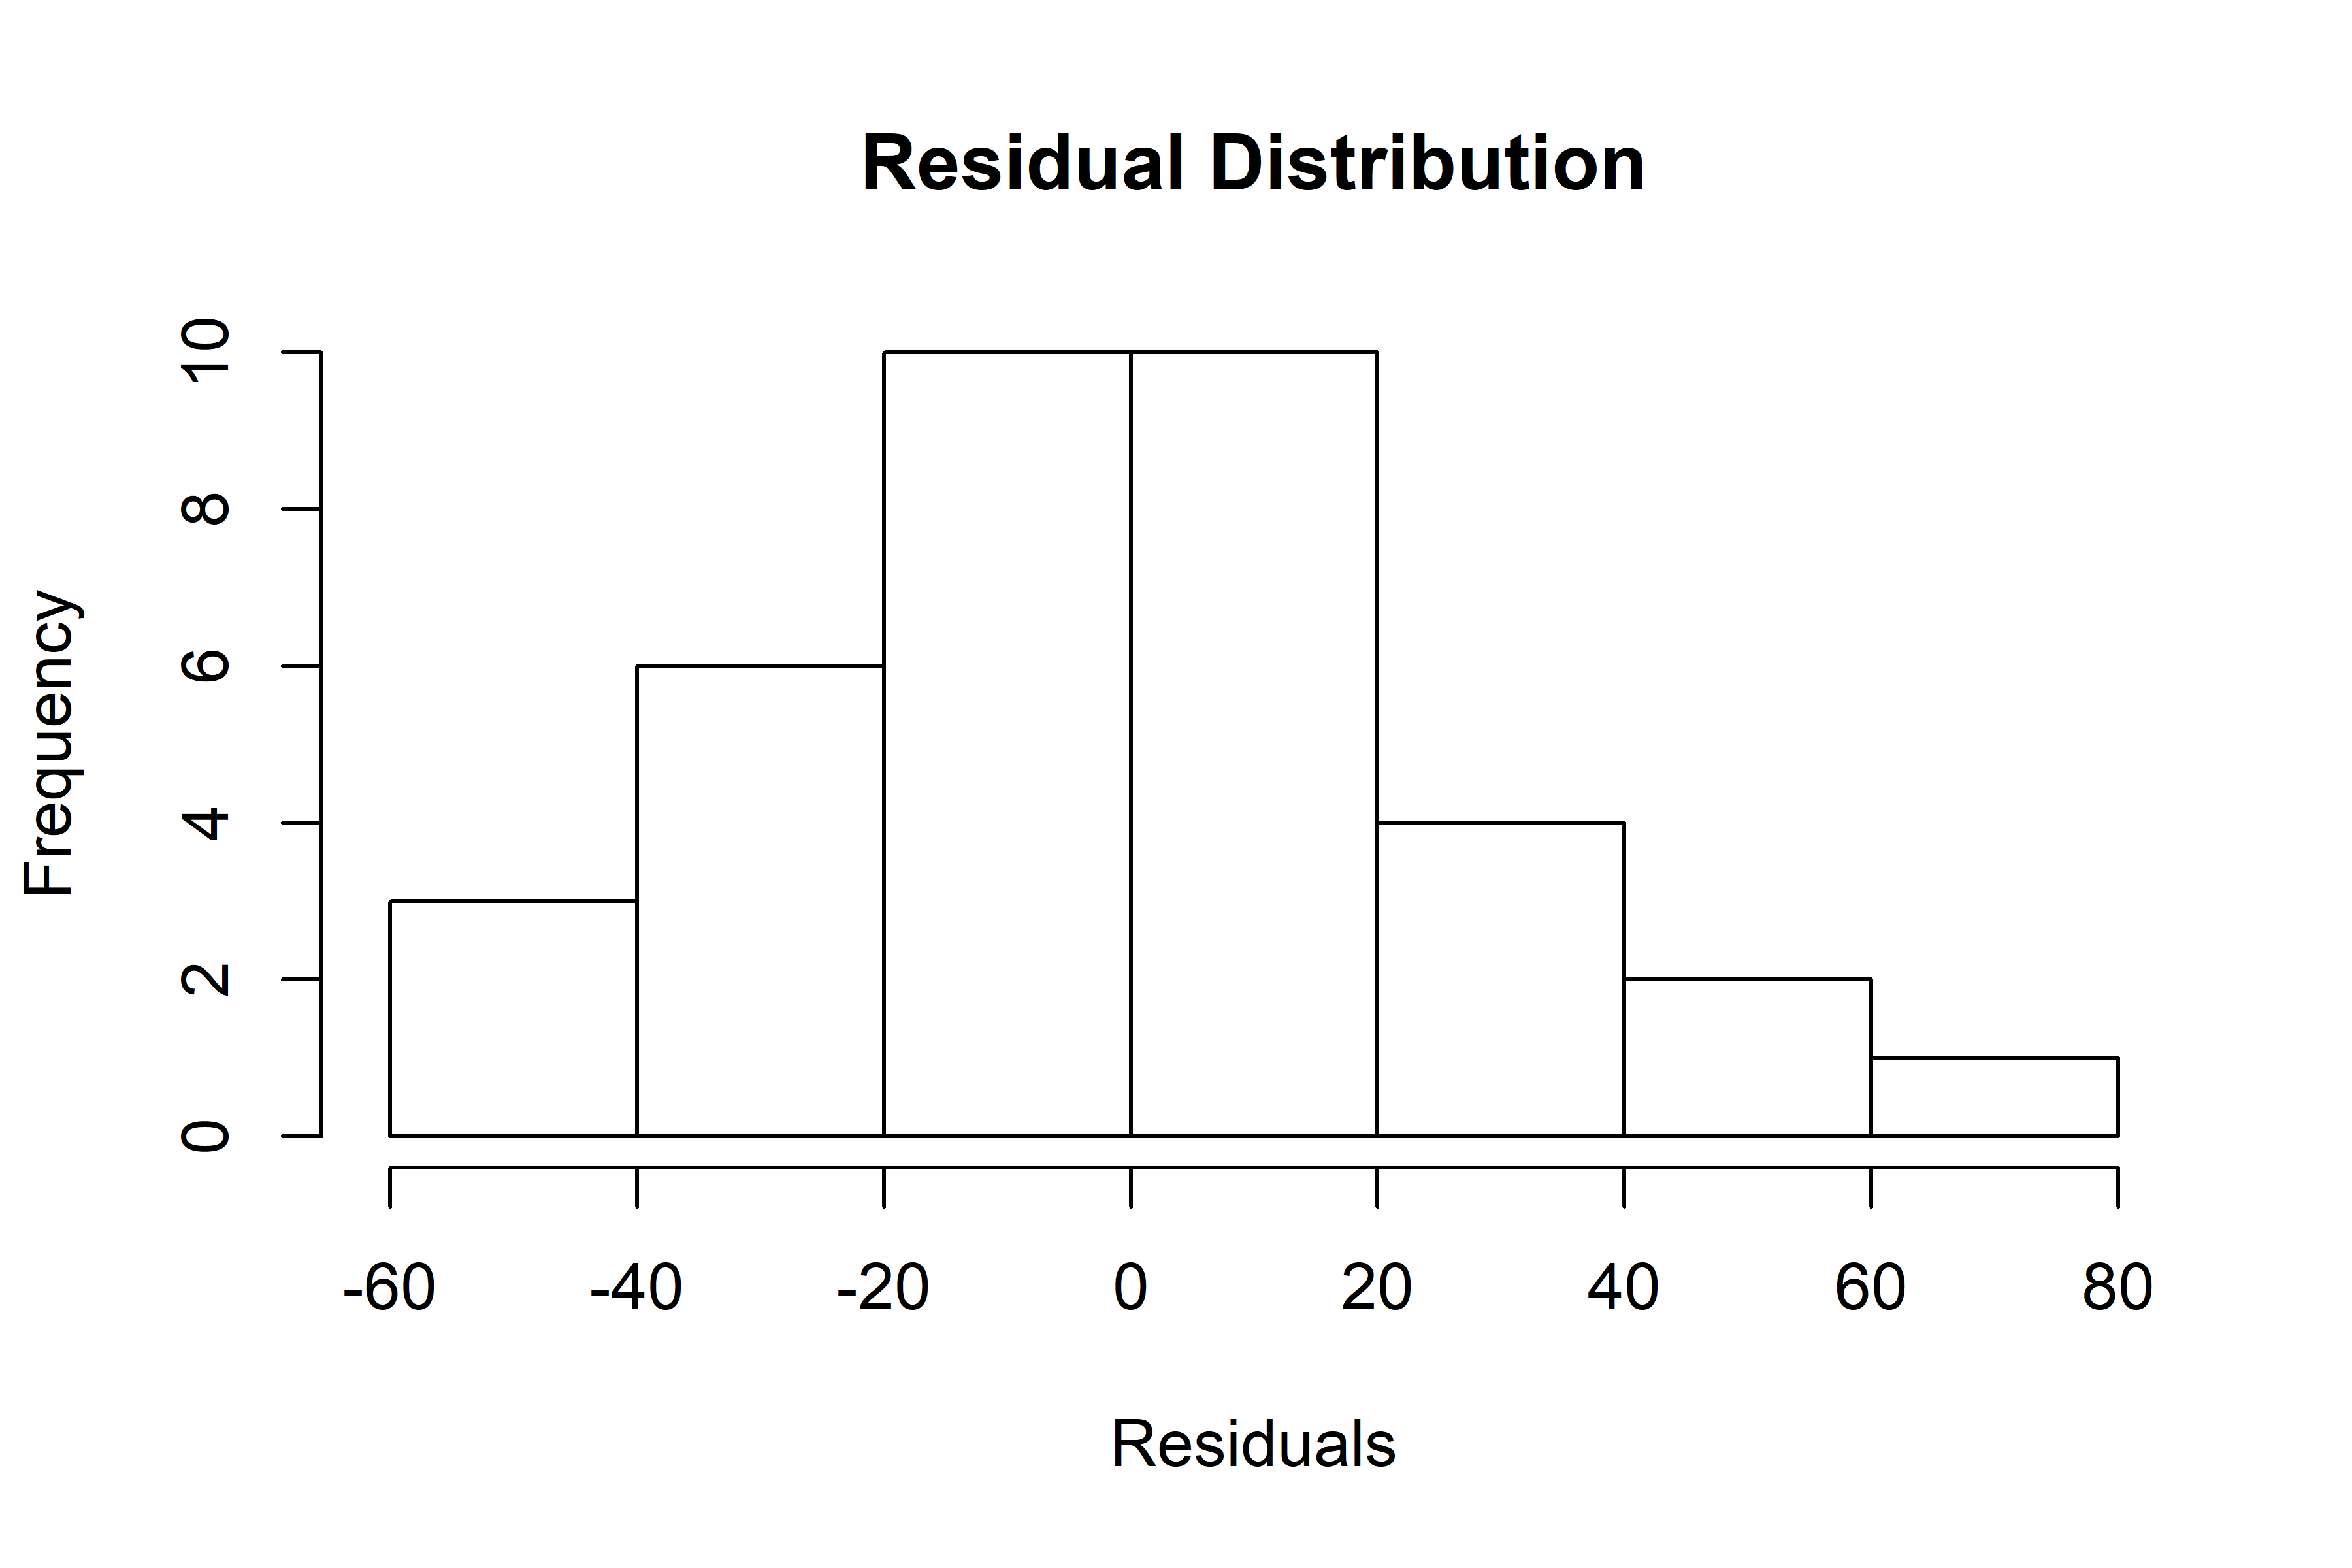
\includegraphics[width=1\textwidth,height=0.25\textheight]{4.png} \\
		\end{minipage}
	}
	\subfigure[Normal QQ Plot]{
		\begin{minipage}[b]{0.43\textwidth}
			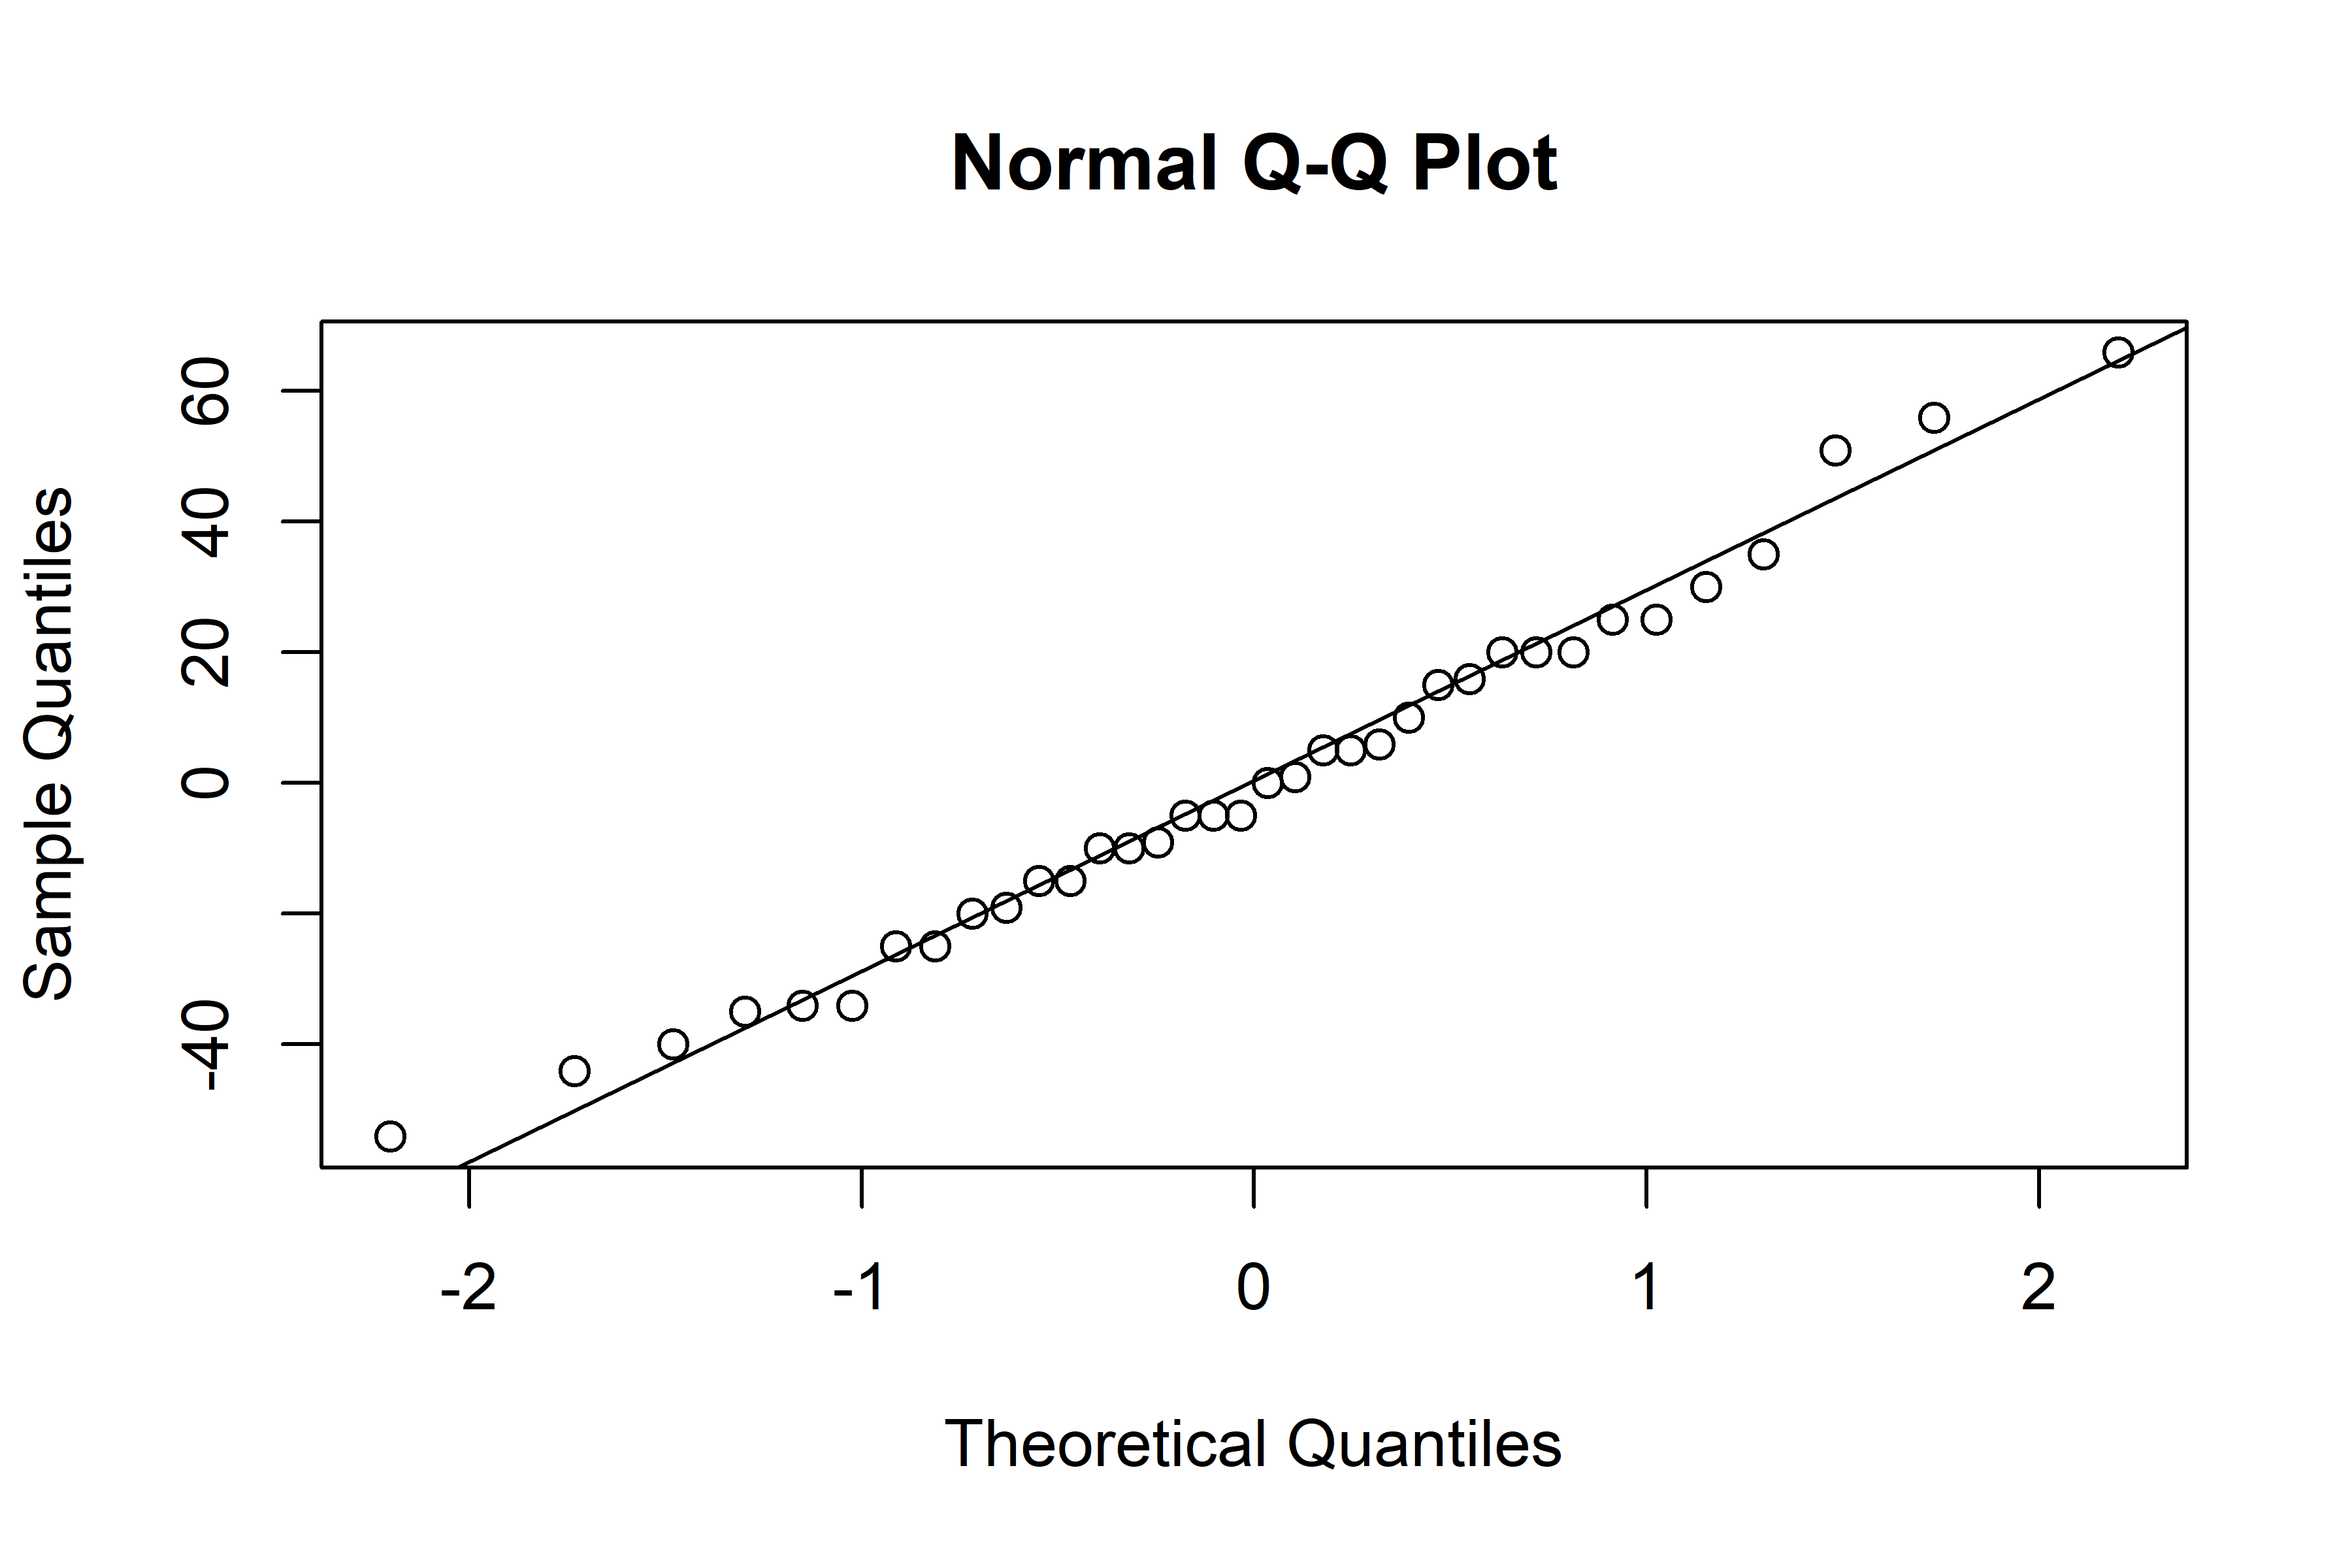
\includegraphics[width=1\textwidth,height=0.25\textheight]{5.png} \\
		\end{minipage}
	}
	\caption{Plots of model diagnostics}
\end{figure}
\subsubsection{Test for equal variance}
We used Modified-Levene test for equal variances. According to R, the p-value is 0.03931. It is small enough for us to reject the null hypothesis at $\alpha=0.05$ and conclude that the variance is not constant. What is more, the plot below also shows the variance is not constant.\par 
Interpret the p-value of Modified-Levene test.
\begin{itemize}
	\item If the variance was constant, we would observe the data or more extreme 3.931\% of the time.
\end{itemize}

\begin{figure}[H]
	\centering
	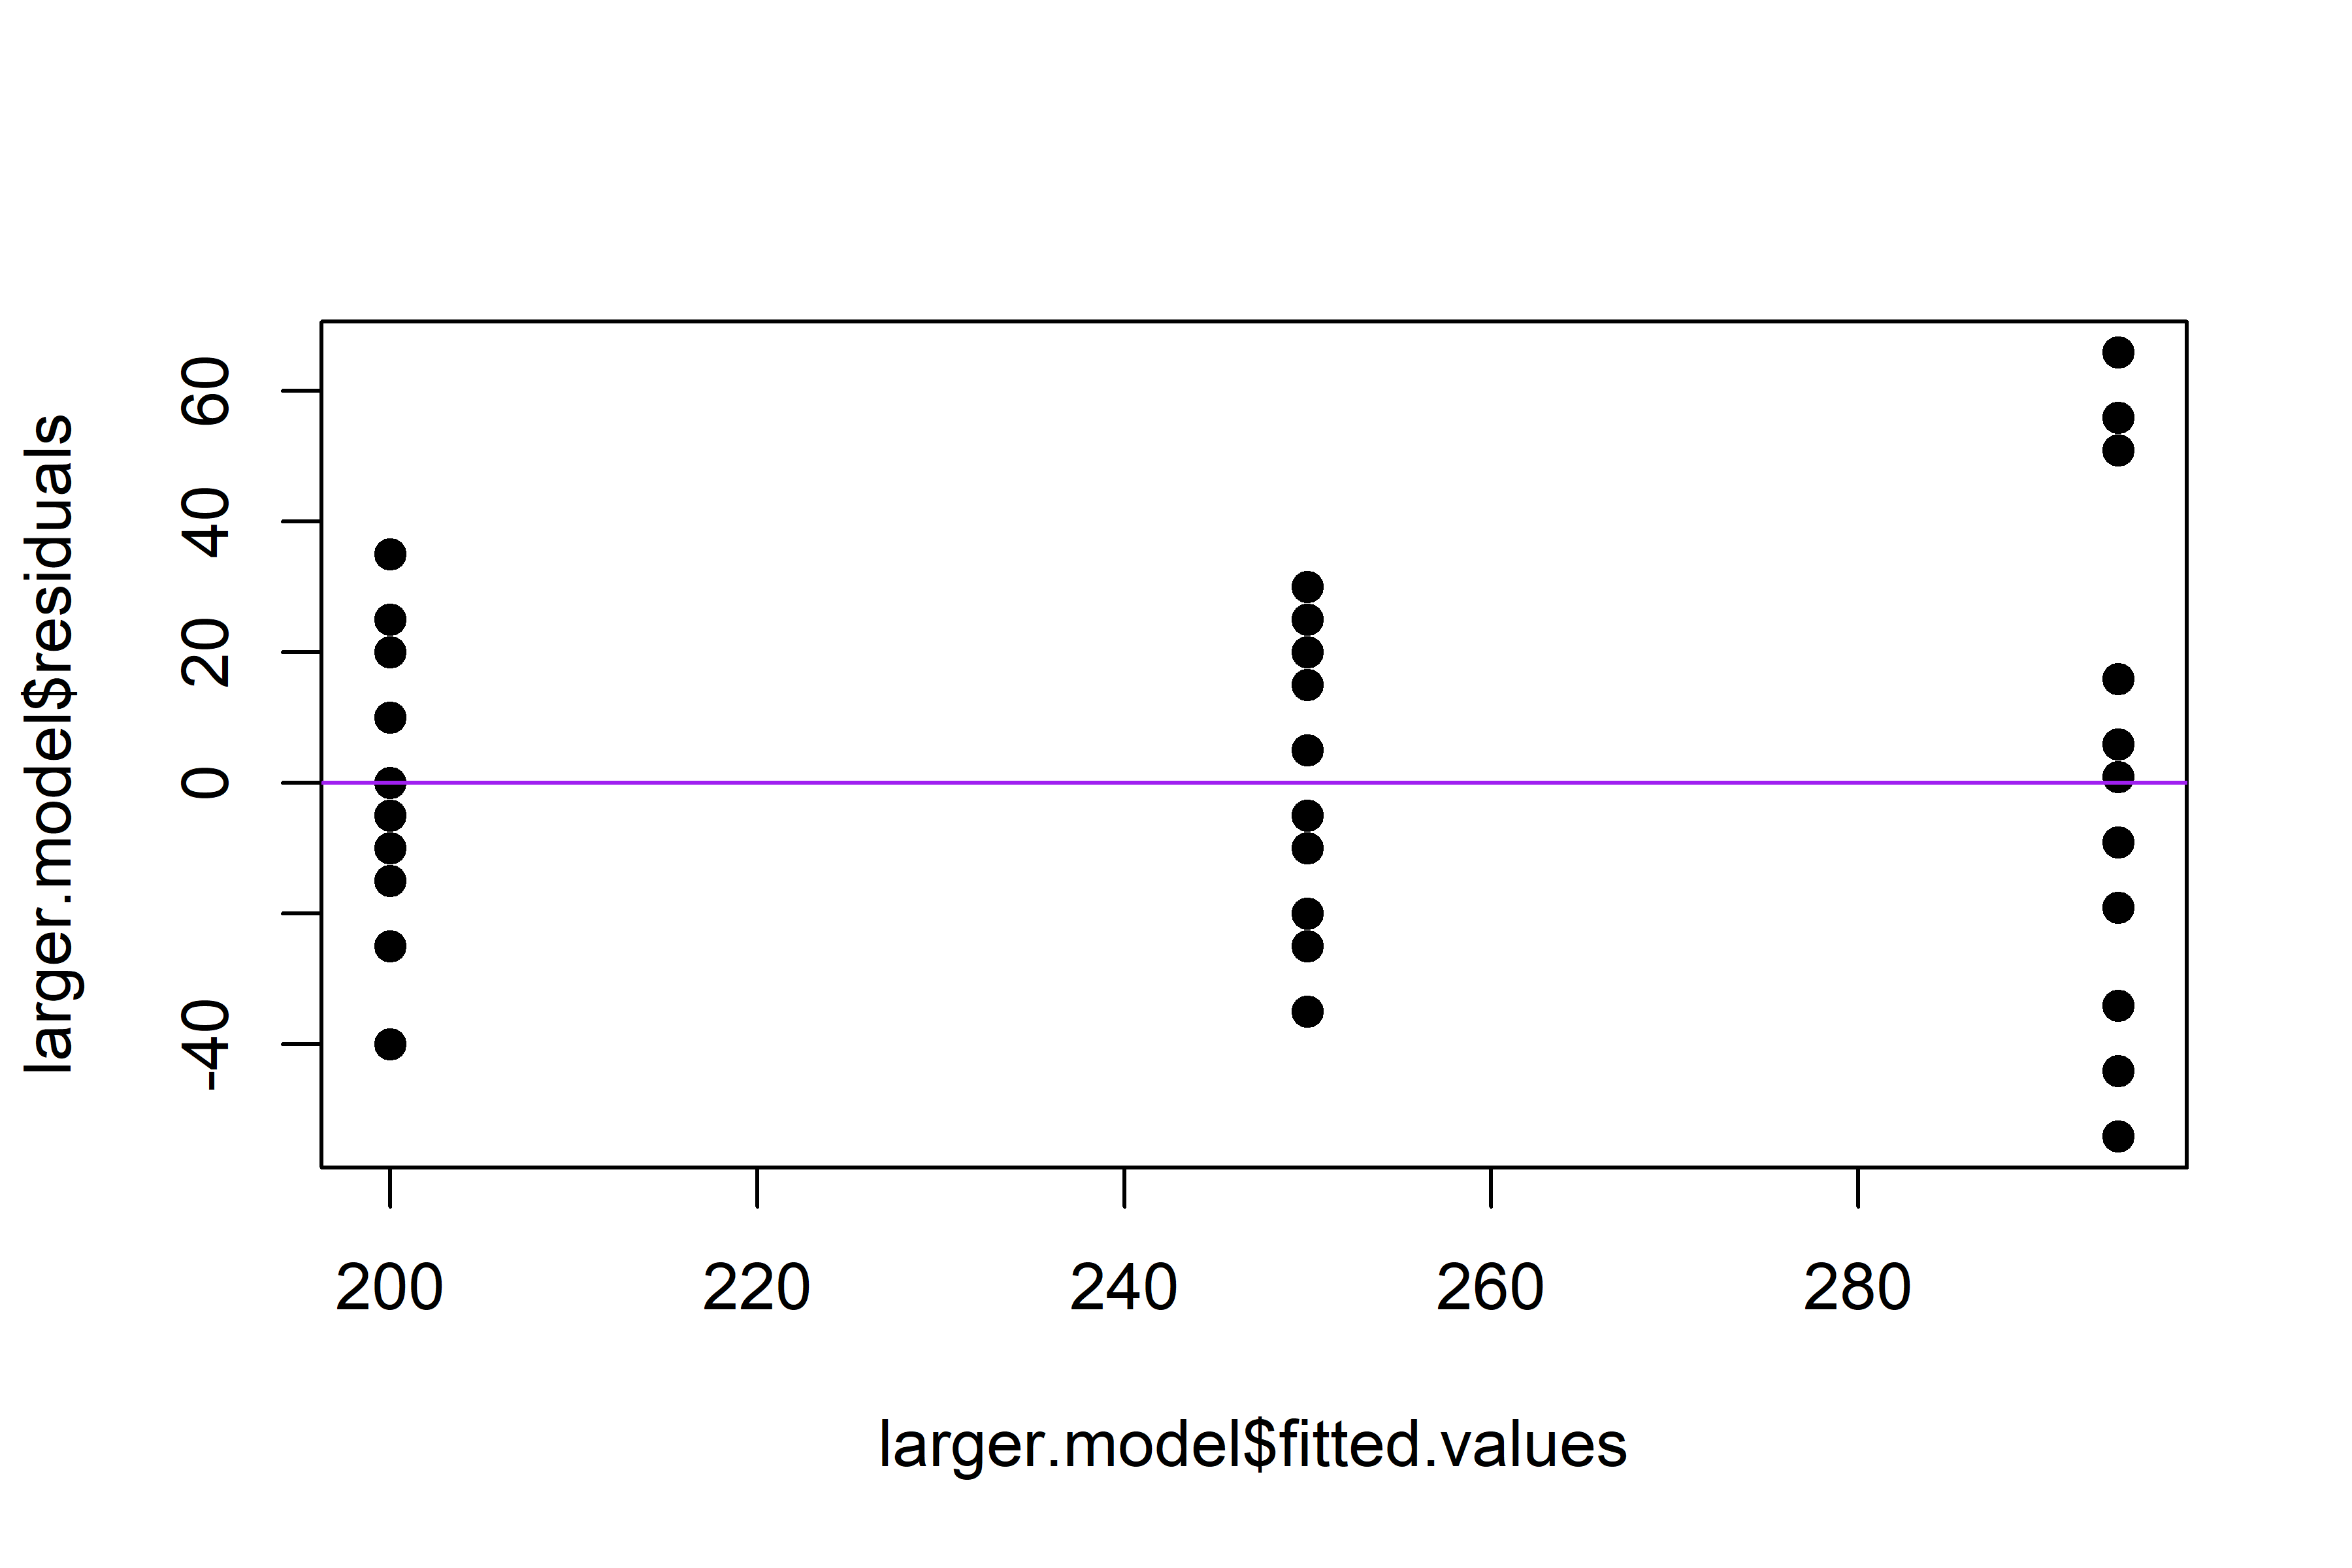
\includegraphics[width=0.6\textwidth,height=0.3\textheight]{6.png}	
\end{figure}
\subsection{Choose cutoff and remove outliers}
Based on the analysis of the standardized residuals in R, using the cutoff based on t-distribution, which is 2.733, there is no outlier in the dataset.
\subsection{Final Model and Predict}
The final model and the estimated $y$ in each group is as follows.
\begin{equation}
\begin{aligned}
\hat{y}_A=\mu_A&=200.0\\
\hat{y}_B\label{key}=\mu_B&=250.0\\
\hat{y}_C=\mu_C&=294.2\\
\end{aligned}
\end{equation}
\subsection{Conclusion}
It is safe for us to conclude that types of grass are of great importance on the weight of cows. For this question, cows that were fed grass C weighed most.\par

\section*{R Appendix}								
\begin{lstlisting}[language=R,caption={R script for Project 2}] 
##### Logistic Regression #####
##### set work directory and load dataset ##### 
setwd("/home/xmy/STA 101/Projects/P2")
prostate <- read.csv("prostate.csv", header = TRUE)
head(prostate, n = 3)

##### load packages #####
library(ggplot2)
library(pROC)
library(EnvStats)
library(bestglm)
library(nnet)
library(LogisticDx)
library(asbio)

##### set default parameters #####
ppi = 600

##### rename columns of datasets #####
names(prostate) = c("Y", "X1", "X2", "X3", "X4", "X5", "X6", "X7")
head(prostate, n = 3)
summary(prostate)

##### define functions #####

##### prostate summary #####

##### preparation of data #####
# filename = "group_boxplot_X1.png"
# png(filename, width=6*ppi, height=4*ppi, res=ppi)
# ggplot(prostate, aes(y=X1, x = as.factor(Y)))+ theme_gray() + geom_boxplot() + ylab("Serum prostate-specific antigen level") + 
#  xlab("Indicator of prostate cancer") 
# dev.off()


##### model selection #####
empty.model = glm(Y~1, data=prostate, family = binomial(link=logit))
full.model = glm(Y~., data=prostate, family = binomial(link=logit))
### Forward stepwise
F.model = step(empty.model, scope = list(lower=empty.model,upper=full.model),trace = FALSE, direction = "forward", criteria = "AIC")
### Backward stepwise
B.model = step(full.model, scope = list(lower=empty.model,upper=full.model),trace = FALSE, direction = "backward", criteria = "AIC")
### Forward/Backward stepwise
FB.model = step(empty.model, scope = list(lower=empty.model,upper=full.model),trace = FALSE, direction = "both", criteria = "AIC")
### Backward/Forward stepwise
BF.model = step(full.model, scope = list(lower=empty.model,upper=full.model),trace = FALSE, direction = "both", criteria = "AIC")
### display selected models
F.model
B.model
FB.model
BF.model

##### final model #####
final.model = glm(Y~X1+X2+X4, data=prostate, family = binomial(link=logit))
summary(final.model)
the.betas = final.model$coefficients
round(the.betas,4)
exp.betas = exp(the.betas)
names(exp.betas) = c("(Intercept)", "exp.X1", "exp.X2", "exp.X4")
round(exp.betas,4)
# display final model
### CI for betas
alpha = 0.05
the.CI = confint(final.model, level = 1 - alpha)
round(the.CI,4)
exp.CI = exp(the.CI)
rownames(exp.CI) = c("(Intercept)", "exp.X1", "exp.X2", "exp.X4")
round(exp.CI,4)


##### if X4 can be dropped #####
model.A = final.model
model.0 = glm(Y~X1+X2, data=prostate, family = binomial(link=logit))
LLA = logLik(model.A)
LL0 = logLik(model.0)
pA = length(model.A$coefficients)
p0 = length(model.0$coefficients)
LR = -2*(LL0-LLA)
p.value = pchisq(LR, df = pA-p0, lower.tail = FALSE)
p.value
# interpret p-value


##### Diagnostics #####
### Pearson residuals
good.stuff = dx(final.model)
pear.r = good.stuff$Pr
std.r = good.stuff$sPr
plot.name = "pearson_std_e.png"
png(plot.name, width=6*ppi, height=4*ppi, res=ppi)
hist(std.r, main = "Pearson Standardized Residuals")
dev.off()
cutoff.std = 3.0
good.stuff[abs(std.r)>cutoff.std]
### dfbeta
df.beta = good.stuff$dBhat
plot.name = "dfbeta.png"
png(plot.name, width=6*ppi, height=4*ppi, res=ppi)
plot(df.beta, main = "Index plot of the change in the Betas")
dev.off()
cutoff.beta = 0.50
good.stuff[df.beta>cutoff.beta]
### dchisq
change.pearson = good.stuff$dChisq
plot.name = "dchisq.png"
png(plot.name, width=6*ppi, height=4*ppi, res=ppi)
plot(change.pearson, main = "Index plot of the change in the Pearson's test-statistic")
dev.off()
cutoff.pearson = 15
good.stuff[change.pearson>cutoff.pearson]

##### ROC and AUC #####
plot.name = "auc.png"
png(plot.name, width=6*ppi, height=4*ppi, res=ppi)
my.auc = auc(final.model$y, fitted(final.model), plot = TRUE)
dev.off()
my.auc
auc.CI = ci(my.auc, level = 0.95)
auc.CI
# interpret auc.CI

##### remove outliers #####
new.prostate  = prostate

# remove outliers
new.prostate = new.prostate[-which(prostate$X1 == 14.880|prostate$X1 == 56.261|prostate$X1 == 9.974),]
the.ratio = (length(prostate$Y)-length(new.prostate$Y))/length(prostate$Y)
the.ratio

##### final best model #####
final.model = glm(Y~X1+X2+X4, data=new.prostate, family = binomial(link=logit))
final.model
summary(final.model)
the.betas = final.model$coefficients
the.betas
exp.betas = exp(the.betas)
names(exp.betas) = c("(Intercept)", "exp.X1", "exp.X2", "exp.X4")
exp.betas
# display final model
### CI for betas
alpha = 0.05
the.CI = confint(final.model, level = 1 - alpha)
the.CI
exp.CI = exp(the.CI)
rownames(exp.CI) = c("(Intercept)", "exp.X1", "exp.X2", "exp.X4")
exp.CI

##### error matrix #####
pi.0=0.30
truth = new.prostate$Y
predicted = ifelse(fitted(final.model)>pi.0,1,0)
my.table = table(truth, predicted)
my.table
sens = sum(predicted == 1 & truth ==1)/sum(truth ==1)
spec = sum(predicted == 0 & truth ==0)/sum(truth ==0)
error = sum(predicted!=truth)/length(predicted)
results = c(sens,spec,error)
names(results) = c("Sensitivity","Specificity","Error-Rate")
results
# interpret error matrix



##### predictive power #####
r = cor(final.model$y, final.model$fitted.values)
r
prop.red = 1-sum((final.model$y - final.model$fitted.values)^2)/sum((final.model$y - mean(final.model$y))^2)
prop.red
# interpret predictive power

##### predict #####
x.star = data.frame(X1 = 10, X2 = 5, X4 = 67)
the.predict = predict(final.model, x.star, type = "response")
the.predict

#### ANOVA ####
cows =read.csv("cows.csv")
head(cows)
ppi = 600
group.means = by(cows$Weight,cows$Grass,mean)  # First argument is Y, second is grouping column/s
png("1.png", width=6*ppi, height=4*ppi, res=ppi)
plot(group.means,xaxt = "n",pch = 19,col = "purple",xlab = "Experiment Group",ylab = "Weight",main = "Average Weight by group",type = "b") #Addinf xaxt = "n" removes the default X axis ticks.
dev.off()

png("2.png", width=6*ppi, height=4*ppi, res=ppi)
boxplot(cows$Weight ~ cows$Grass, main = "Weight by group",ylab = "Weight")
dev.off()

group.means = by(cows$Weight,cows$Grass,mean)
group.sds = by(cows$Weight,cows$Grass,sd)
group.nis = by(cows$Weight,cows$Grass,length)
the.summary = rbind(group.means,group.sds,group.nis)
the.summary = round(the.summary,digits = 4)
colnames(the.summary) = names(group.means)
rownames(the.summary) = c("Means","Std. Dev","Sample Size")
the.summary

library(asbio)
options(scipen = 8)
larger.model = lm(Weight ~ Grass , data = cows)
smaller.model = lm(Weight ~1 , data = cows)
anova.table = anova(smaller.model, larger.model)
anova.table
bonfCI(cows$Weight,cows$Grass, conf.level = 0.95)
bonfCI

p = length(larger.model$coefficients) #Counts the number of betas
alpha = 0.01 # You may change this to whatever you like
t.cutoff = qt(1- alpha/2, n-p)
ei.s = larger.model$residuals/sqrt(sum(larger.model$residuals^2)/(length(larger.model$residuals) - length(larger.model$coefficients)))
outliers = which(abs(ei.s) > t.cutoff)
outliers
t.cutoff

png("3.png", width=6*ppi, height=4*ppi, res=ppi)
plot(larger.model$residuals,main = "Residual index plot",xlab = "Index",ylab = "residuals",pch = 19, col = "purple")
dev.off()
par(mfrow=c(1,2))
png("4.png", width=6*ppi, height=4*ppi, res=ppi)
hist(larger.model$residuals,main = "Residual Distribution",xlab = "Residuals")
dev.off()
png("5.png", width=6*ppi, height=4*ppi, res=ppi)
qqnorm(larger.model$residuals)
qqline(larger.model$residuals)
dev.off()

shap.test = shapiro.test(larger.model$residuals)
shap.test$p.value
ML.test = modlevene.test(larger.model$residuals,cows$Grass)
ML.test$'Pr(>F)'
png("6.png", width=6*ppi, height=4*ppi, res=ppi)
plot(larger.model$fitted.values,larger.model$residuals,pch = 19)
abline(h= 0 , col = "purple")
dev.off()
\end{lstlisting} 



\end{document}